Even after applying WW selection and the \mHi-dependent selection to suppress 
backgrounds, there are events that survive these selections. In order to extract 
the signal component from data, precise estimation of these residual backgrounds 
along with their uncertainty is essential. 

Figure~\ref{fig:bkgcomposition} shows the background composition in the cut-based 
analysis on the top and in the shape-based analysis on the bottom. 
The total background yield is normalized to 1, so the plots show only relative 
contribution of each background. To have a sense of the size of the signal, 
\mHi=125~\GeV\ contribution(red) is overlaid. The yields are after
applying all selections; \mHi-depedent selection on top of WW selection for 
the cut-based plot and $60<\mT<280~\GeV$ and $12<\mll<200~\GeV$ cuts on top of 
WW selection for the shape-based plot. All final states are shown for the
cut-based plot while only are shown \DF\ 0-jet and 1-jet final states  
for the shape-based plots where the method is applied. 
In the 0-jet category, \ww\ is the dominant process in both \DF\ and \SF\ 
categories, and \Wjets\ and \dyll\ follow in the \DF\ and \SF\ categories,
repectively. 
In the 1-jet category, \ww\ and \topbkg are almost equally dominant both \DF\ and \SF\
categories, and \Wjets\ and \dyll\ follow in the \DF\ and \SF\ categories,
repectively.
%
\begin{figure}[htp] 
\centering 
\begin{tabular}{c} 
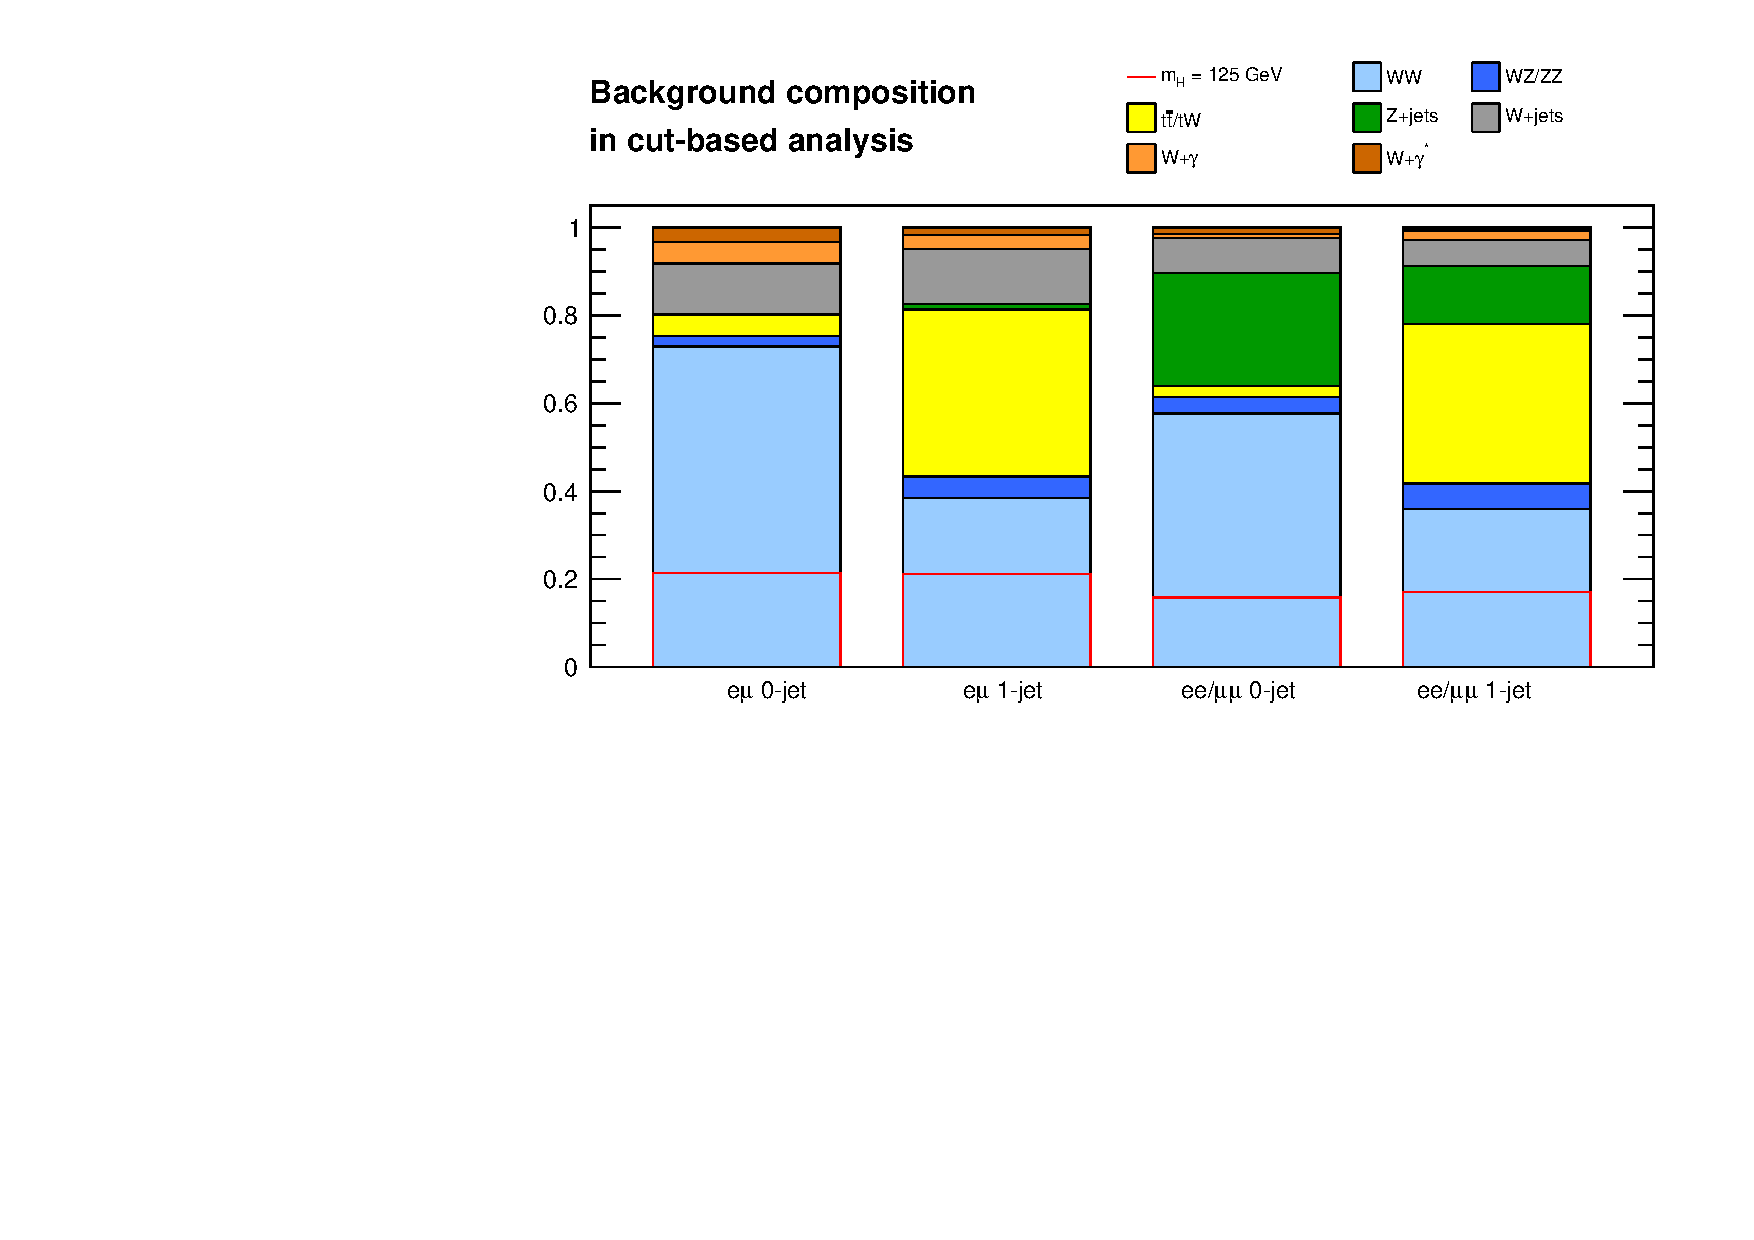
\includegraphics[width=0.9\textwidth]{figures/Bkgcomposition_cutbased.pdf} 
\\
\\
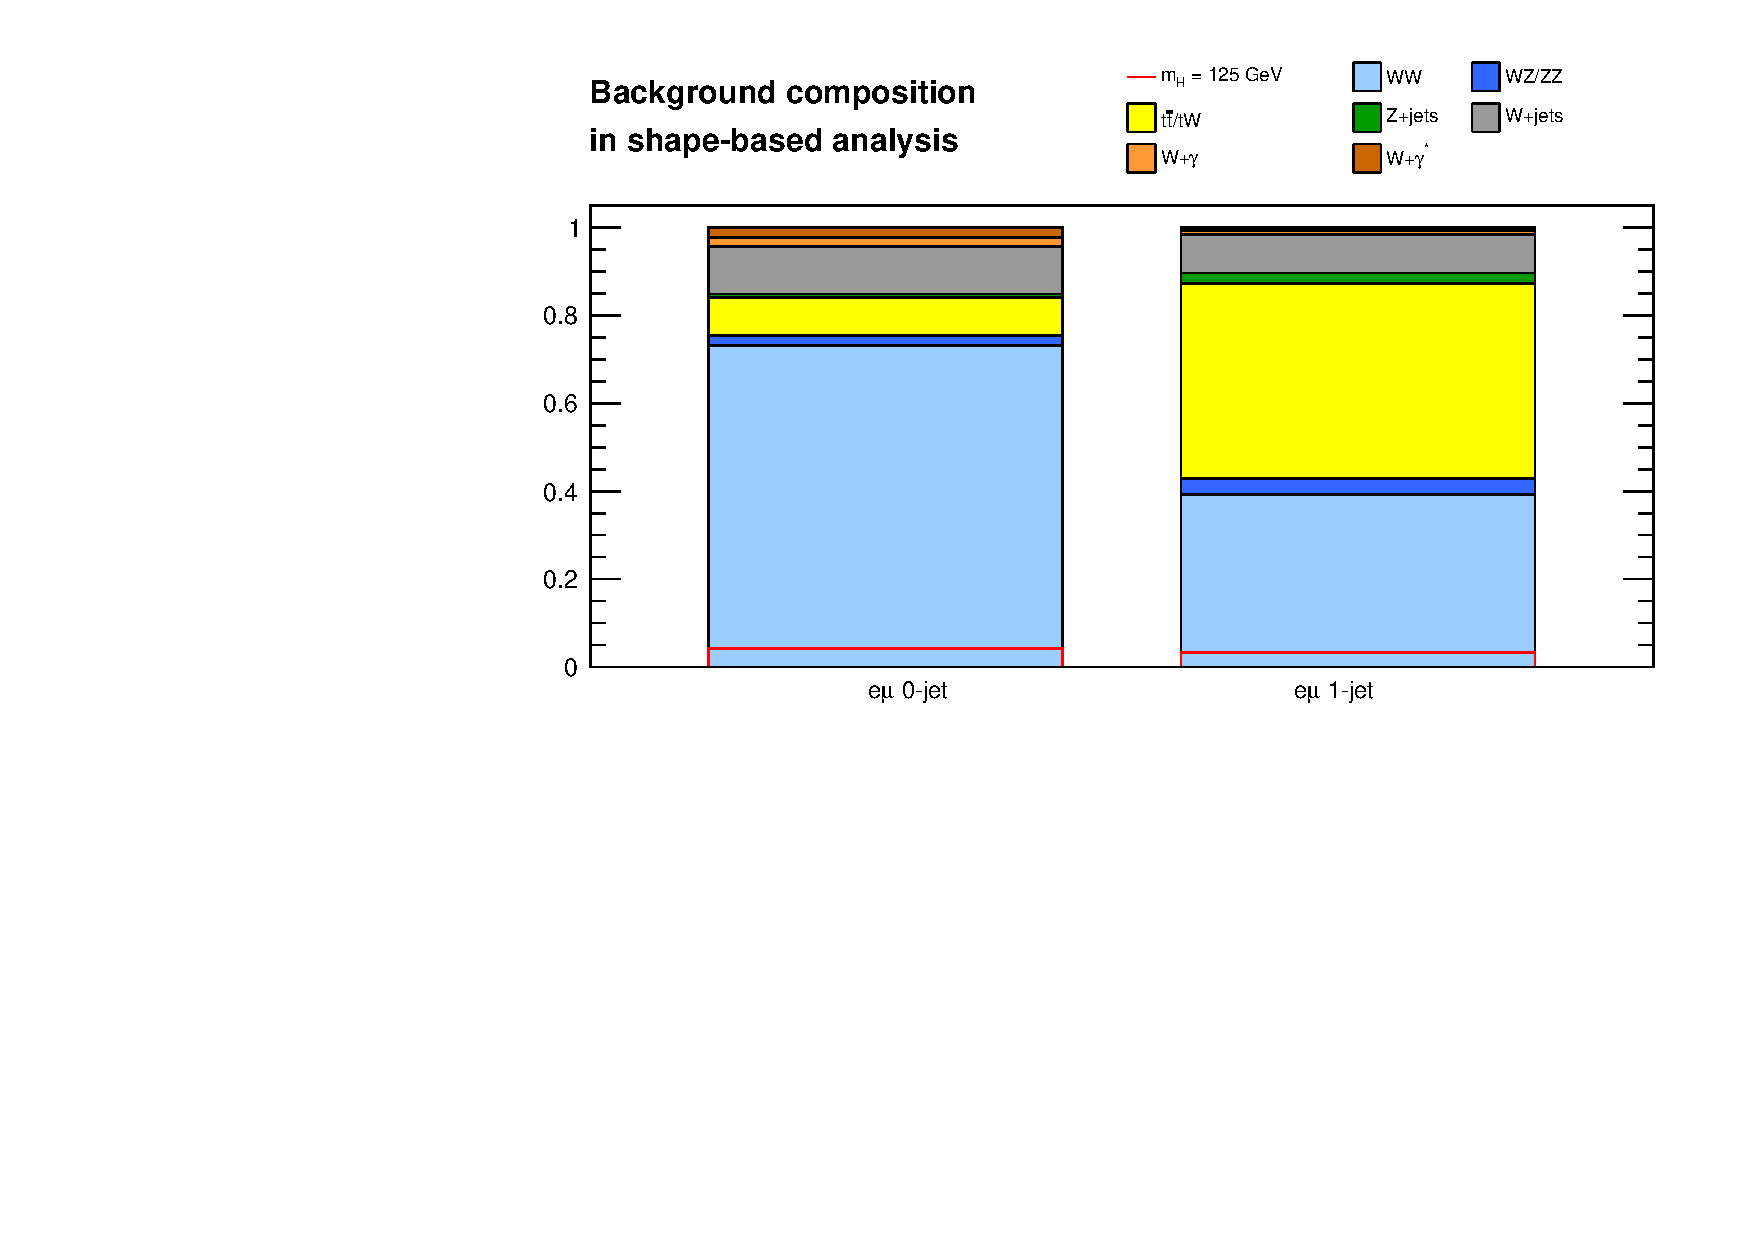
\includegraphics[width=0.9\textwidth]{figures/Bkgcomposition_2d.pdf} 
\end{tabular} 
\caption{Background composition for cut-based(top) and shape-based analyses(bottom) 
for the \mHi=125~\GeV\ hypothesis. Signal contribution is overlaid. 
For the cut-based plot the \mHi\ selection on top of 
WW selection is applied and the plot shows all final states. 
For the shape-based plot \mT\ and \mll\ cuts to construct templates are applied 
on top of WW selection and the plot shows \DF\ 0-jet and 1-jet final states 
where the shape-based method is applied. 
} 
\label{fig:bkgcomposition} 
\end{figure} 

The methods to estimate the contribution of each background depend on the process. 
The best way to do it is to measure it using data control samples, which is 
called ``data-driven method" which will be discussed more in the next paragraph. 
For most of the main backgrounds, we do data-driven estimations using dedicated
data control samples. For the rest of the process, we take it from MC.
Table~\ref{tab:overview_bkgest} shows which background is estimated by 
data-driven methods and which is taken from MC. 

%
\begin{table}[htp] 
\begin{center} 
\vspace{0.5cm}
\begin{tabular}{c}   

\begin{tabular}{c|c|c|c|c|c}   
\hline 
Background     & \qqww & \topbkg & \dyll & \Wjets & \wgammastar  \\
\hline 
\hline 
Method         & data & data & data & data & data \\ 
\hline 
\end{tabular} 
\\
\\
\begin{tabular}{c|c|c|c}   
\hline 
Background     & \ggww & \wgamma & \vv \\
\hline 
\hline 
Method         & MC & MC & MC \\ 
\hline 
\end{tabular} 

\end{tabular} 

\vspace{0.5cm}
\caption{Method of background estimation for each background. Major backgrounds 
are estimated by data-driven methods and  \ggww,  \wgamma\ and  \vv\ are taken 
from simulation.} 
\label{tab:overview_bkgest} 
\end{center} 
\end{table} 

The basic idea of data-driven method is to measure the ratio($\epsilon$) of the number of events  
passing the final selection($N_{SR}^{independent}$) to the number of events passing an inverted 
selection($N_{CR}^{independent}$) using data samples which is independent of the data samples 
used to extract signal events. The SR and CR in the subscript stand for signal region 
which corresponds to the final selection for signal extraction 
and control region which is the region where one or more requirements are inverted. 
The independent sample can be either data or MC. Then, we apply the ratio($\epsilon$)
to the number of events in the control sample passing the inverted selection($N_{CR}^{control}$).
Note that the control region is where some of the selections are inverted. 
All this can be written as an equation, 
\begin{eqnarray} 
N_{SR} = \epsilon \times N_{CR}^{control}.
\end{eqnarray} 

When measuring $\epsilon$ or $N_{CR}^{control}$, we need to subtract 
the contributions from other processes to measure only process we 
are interested in. This results in dependencies between estimations 
of the backgrouns processes. Fig.~\ref{fig:bkgest_dependency} shows 
the dependency of data-driven background estimation. 
The \dyll\ and \Wjets\ do not depend on the other data-driven estimations. 
The estimation of \wgammastar\ depends on the estimation of \Wjets. 
The estimation of \topbkg\ depends on \wgammastar, \dyll\ and \Wjets. 
The estimation of \qqww\ depends on \wgammastar, \dyll,  \Wjets\ and \topbkg. 
These dependencies natually decide in which order background processes
need to estimated. The \dyll\ and \Wjets\ are done first, 
and \wgammastar, \topbkg\ and \qqww\ follow. This chapter will discuss 
the details following the above order. 
\begin{figure}[ht!] 
\centering 
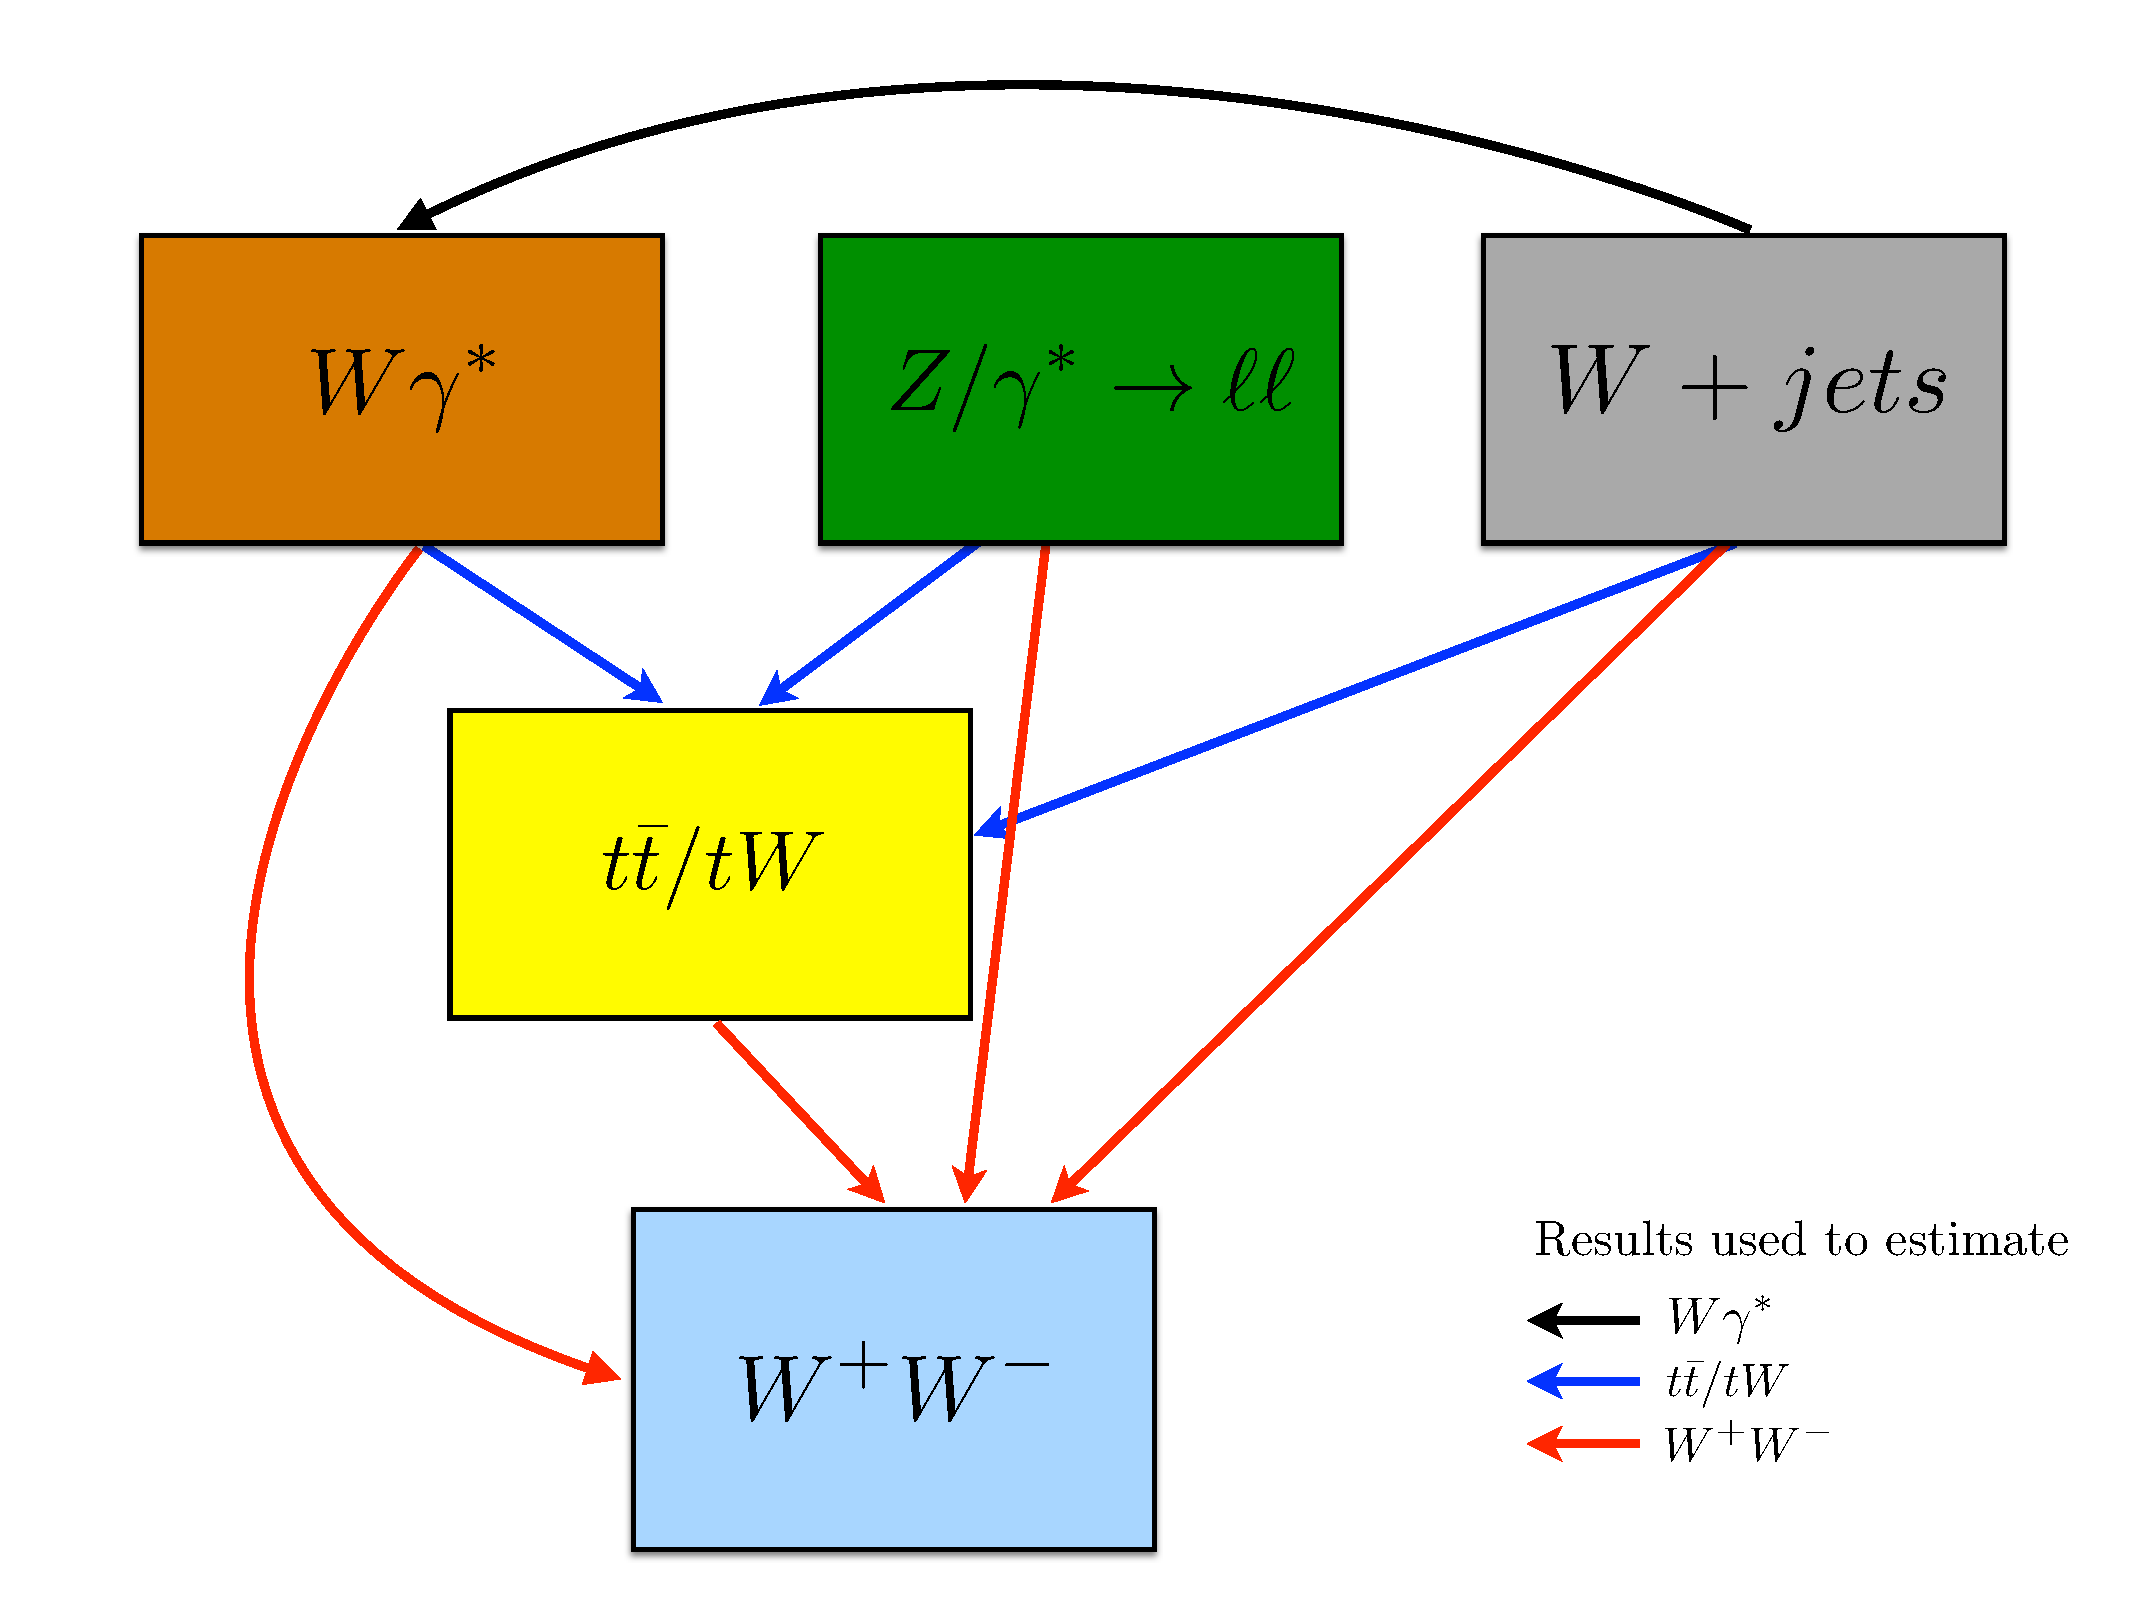
\includegraphics[width=0.99\textwidth]{figures/bkgest_schematic.pdf} 
\caption{Dependency of data-driven estimations.} 
\label{fig:bkgest_dependency} 
\end{figure} 

%%%%%%%%%%%%%%%%%%%%%%%%%%
\section{ \dyll }

\dyll\ is one of the main backgrounds in the \SF\ category.   
\dyll\ events do not have intrinsic \met. But, any mis-measurements can 
lead to fake(instrumental) \met, of which mis-measurement of jet momentum dominates.  
The expected contribution of \dyll\ in the signal region is estimated by 
counting events near the Z mass ($|\mll - m_Z| < 7.5~\GeV$
\footnote{Tighter mass window than Z veto requirement in the WW selection is chosen
to reduce other background contributions}) in data, subtracting 
the contribution from other processes, and scaling it by the ratio (\routin) 
which is defined as the ratio of events outside of Z peak to the events inside
of Z peak with looser DY MVA requirement. In equation, this can be written by 
\begin{eqnarray} 
N(ll)^{DY}_{SR} 
= 
%\begin{array}{ccc} \multicolumn{2}{c}{\displaystyle 
\left( N(ll)_{CR}^{data} - 0.5 \times N(e\mu)_{CR}^{data} \times k_{ll} - N_{CR}^{\vv, MC} \right) 
%} & \\ & \multicolumn{2}{c}{\hspace{8cm} \displaystyle
\times R(ll)_{out/in}
%} \end{array}   
\end{eqnarray} 
where 
\begin{itemize}
\item $ll$ : $ee$ or $\mu\mu$ 
\item $N(ll)^{DY}_{SR}$ : expected \dyll\ contribution in the signal region(SR) 
\item $N(ll)_{CR}^{data}$ : number of $ll$ data events in the control region(CR) which is 
      under the Z peak ($|\mll - m_Z| < 7.5~\GeV$)  
\item $N(e\mu)_{CR}^{data}$ : number of $e\mu$ data events in the control region(CR) which is 
      under the Z peak ($|\mll - m_Z| < 7.5~\GeV$)  
\item $k_{ll}$ : efficiency correction for $e\mu$ events,  \\
      $\displaystyle k_{ee} = \sqrt{\frac{N(ee)_{in}^{loose}}{N(\mu\mu)_{in}^{loose}}}$  and   
      $\displaystyle k_{\mu\mu} = \sqrt{\frac{N(\mu\mu)_{in}^{loose}}{N(ee)_{in}^{loose}}}$,
      measured with loose selection ($\minpmet > 20~\GeV$) 
\item $N_{CR}^{\vv, MC}$ : contribution from \vv\ events estimated in MC
\item $R(ll)_{out/in}$ : \routin\ value measured in data with looser DY MVA selection
\end{itemize}
The number of events in the CR($N(ll)_{CR}^{data}$) is corrected by subtracting
\vv\ and $e\mu$ contribution($N(e\mu)_{CR}^{data}$) which is dominated by \topbkg\ with 
efficiency correction between \SF\ and $e\mu$. The lepton efficiency does not depend 
on the DY MVA requirement, so we can measure it without DY MVA requirement 
to get more statistics. The statistical uncertainty on the lepton efficiency 
measured with the events under the Z peak is at the level of \textcolor{red}{XX} \%,
much smaller than the dominant systematic uncertainty. 
The \vv\ contribution is taken from MC because they have real \met, 
and real \met\ is well-modelled by simulation.
\textcolor{blue}{The reason why \vv\ is considered separately from \dyll
is that the extrapolation from CR to SR can be different for the two 
processes once the full selection is applied.}  
For the \vv\ contribution in the CR, we assign 10 \% of systematic uncertainty.  
\textcolor{red}{where does this 10\% come from?} 

The $R(ll)_{out/in}$ value is measured in data with looser DY MVA requirement. 
The assumption is that the \routin value does not change as a function of 
DY MVA, which is expected because DY MVA is dominantly dependent on \met\ 
and \met\ in \dyll\ events mostly comes from jet momentum mismeasurement, 
which is weakly correlated to the lepton energy/momentum from which 
\mll\ is calculated. So, we divide the DY MVA output into 4 bins
([-0.9,-0.85], [-0.85,-0.60], [-0.60,WP], [WP,1.0]) where WP 
is 0.88 for 0-jet and 0.84 for 1-jet and measure the 
\routin using the bin closest to the signal region in order to get the 
sample with similar kinematics as the signal region events.  
\begin{figure}[ht!] 
\centering 
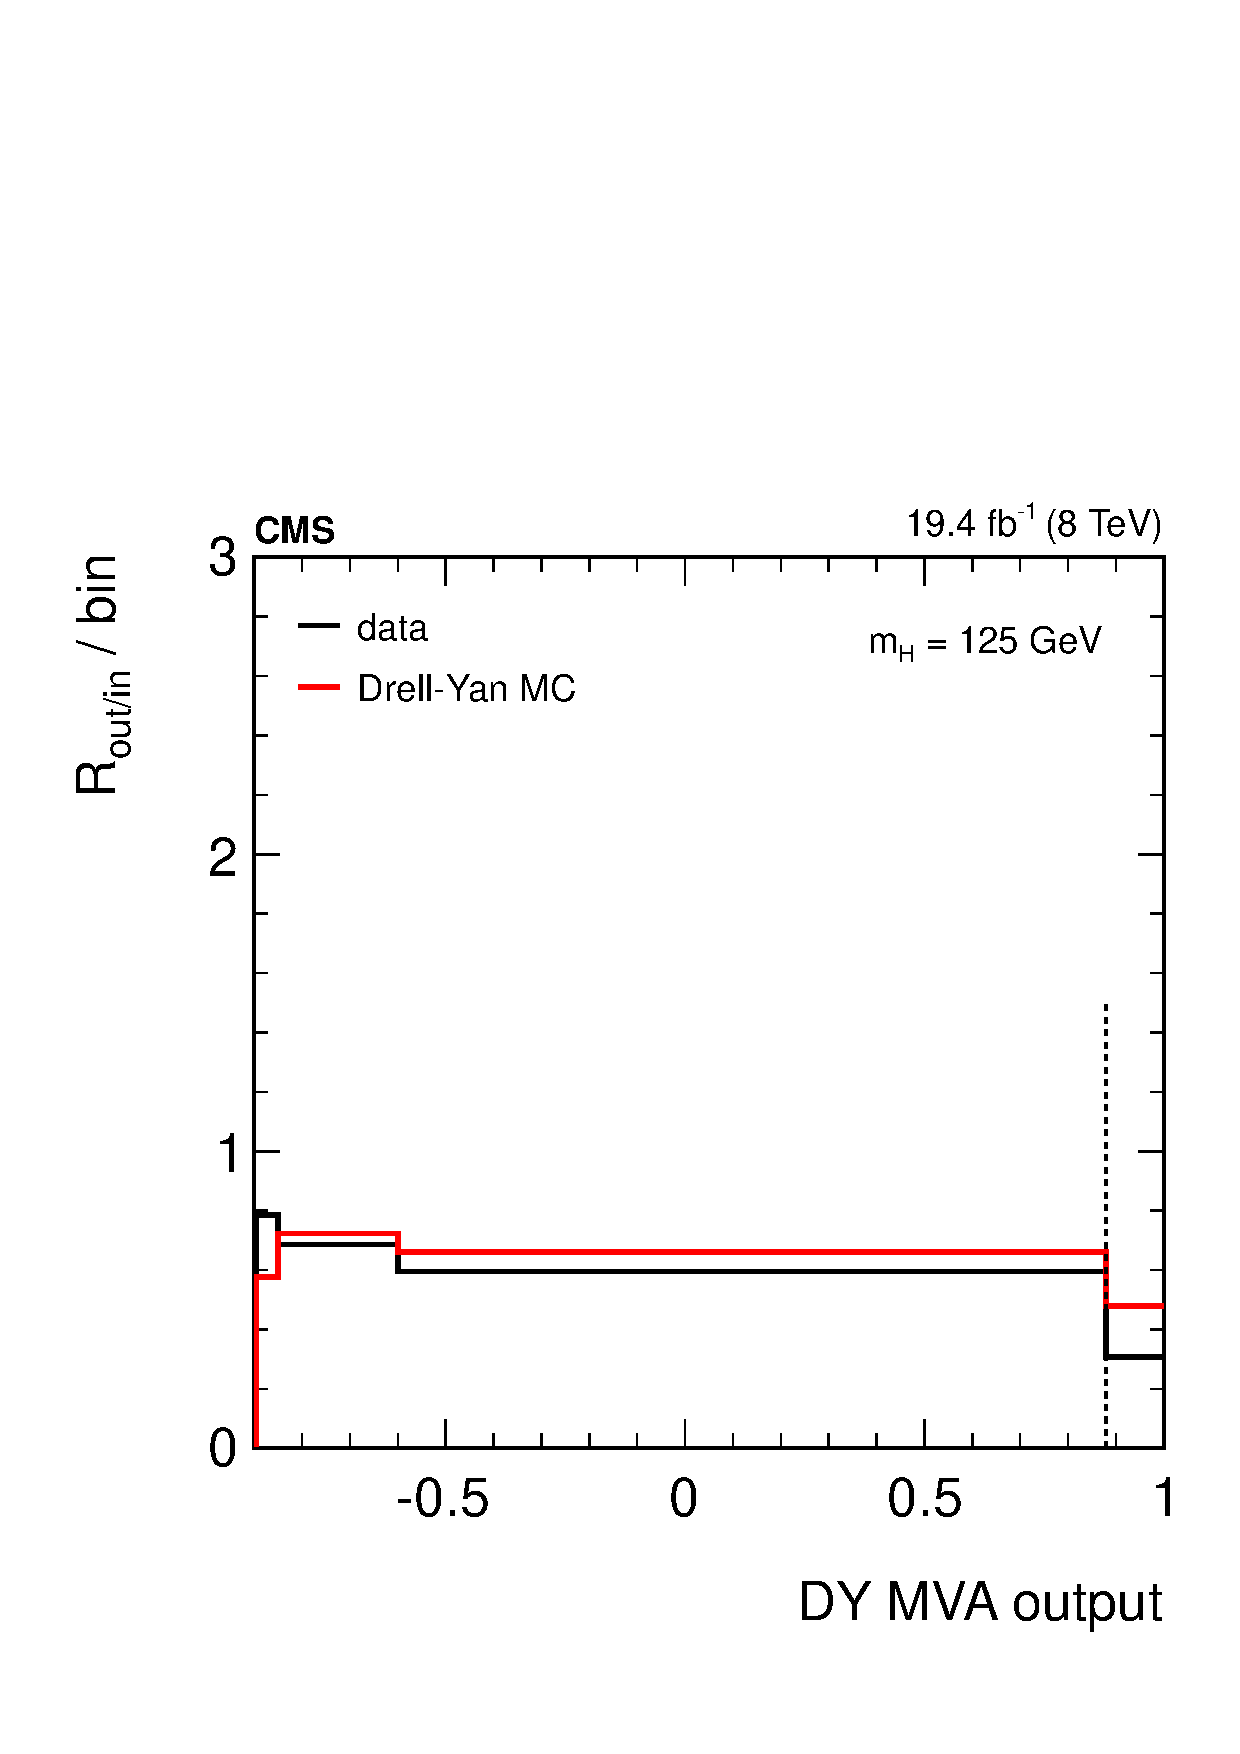
\includegraphics[width=0.5\textwidth]{figures/Routin_0Jet_mH125_19467pb_dy.pdf} 
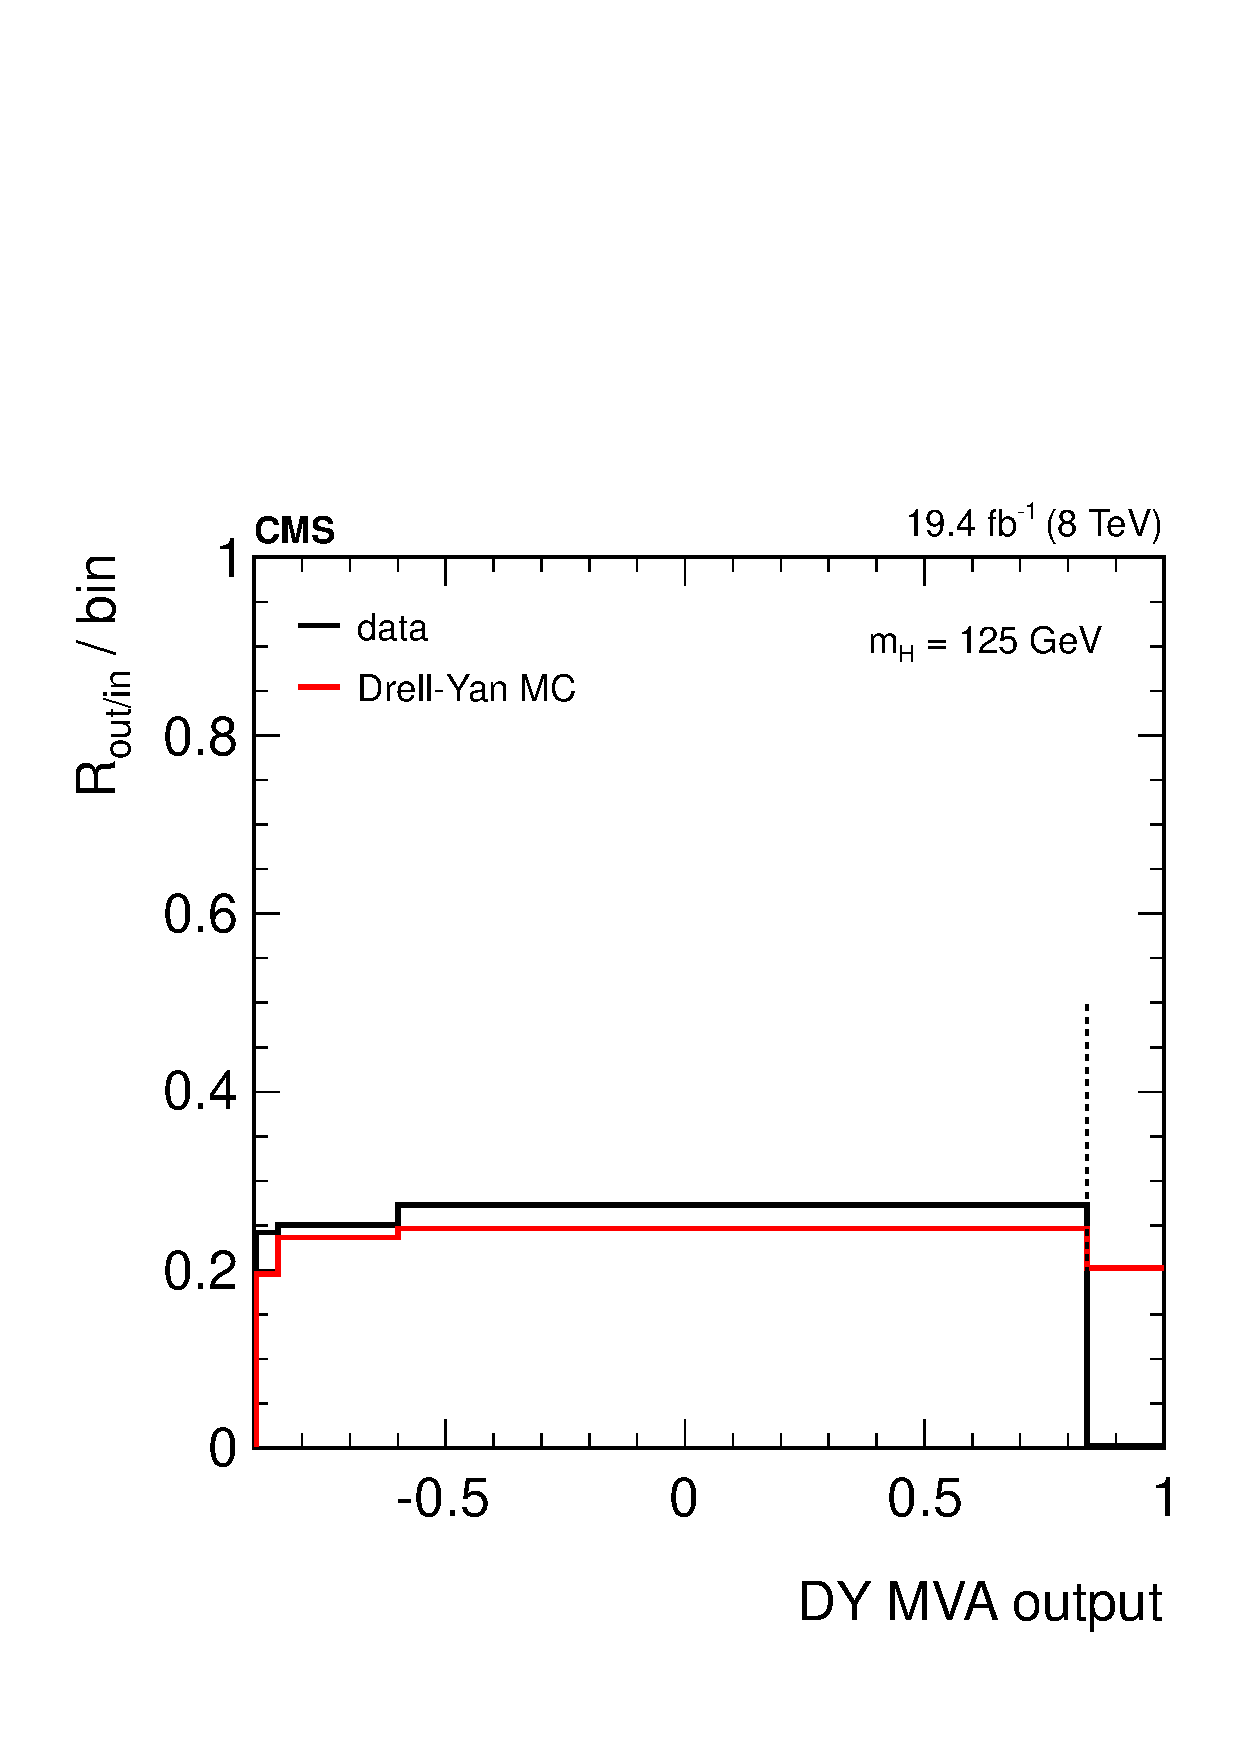
\includegraphics[width=0.5\textwidth]{figures/Routin_1Jet_mH125_19467pb_dy.pdf} 
\caption{\routin\ values as a function of DY MVA output for 0-jet and 1-jet categories
for \mHi=125~\GeV\ analysis. 
The black is from data subtracting \vv\ contribution and the red is from MC. 
The vertical dotted lines show the cut for signal region.} 
\label{fig:routin_mh125} 
\end{figure} 
Fig.~\ref{fig:routin_mh125} shows \routin\ divided by 4 bins for 0-jet and 1-jet for 
\mHi = 125~\GeV\ analysis. The fourth bin, located after the vertical dotted lines, 
corresponds to the signal region. The results using data subtracting \vv\ component 
and using MC are drawn as black and red. The both results show that \routin\ is almost 
flat as a function of DY MVA output. 

The systematic uncertainty comes from the ``unflatness" of the \routin, 
the largest difference between the third bin and the other bins.
\textcolor{red}{how large is this?} In addition, 
there is an alternate method to estimate \dyll\ using $\gamma$ + jets data sample. 
The difference between this method and \routin\ method in 
the extrapolation from CR to SR is about 30 \%. 
We take the maximum of the two as the final systematics of the estimation. 

At the end we merge $ee$ and $\mu\mu$ to get more statistics. 
The tab.~\ref{tab:dy_wwlevel} shows the final estimation at WW level.
The tab.~\ref{tab:dy} 
shows the final estimation of \dyll\ at all \mHi\ hypotheses up to 300 \GeV. 
After 300 \GeV, the $N_{out}(data)/N_{out}(MC)$ scale factor for WW selection 
is applied. 

%%%%%%%%%%%%%%%%%%%%%%%%%%%%%% 
\begin{table}
\begin{center}
\small
\begin{tabular}{c c c c c c}
\hline
       nJets & $N_{in}$(data)        & $R_{out/in}$        & $N_{out}$(data)  & $N_{out}$ (MC) \\ 
\hline
0 & $775.16\pm74.47$ & $0.28\pm0.01\pm0.08$ & $218.64\pm21.53\pm65.59$ & $34.64\pm9.56$ \\
1 & $350.69\pm38.00$ & $0.25\pm0.01\pm0.08$ & $89.20\pm9.83\pm26.76$ & $21.05\pm7.16$ \\
\hline
\end{tabular}
\caption{The Drell-Yan estimation in the same flavor final state at WW selection level, using the DYMVA.}
\label{tab:dy_wwlevel}
\end{center}
\end{table}

%%%%%%%%%%%%%%%%%%%%%%%%%%%%%%
\begin{table}
\begin{center}
\small
\begin{tabular}{c c c c c c}
\hline
\hline
\multicolumn{5}{c}{0-jet} \\
\hline
mass & $N_{in}$(data)        & $R_{out/in}$        & $N_{out}$(data)  & $N_{out}$ (MC) \\ 
\hline
%\vspace{-3mm}  \\
115 \GeV & $145.94\pm15.08$ & $0.31\pm0.01\pm0.09$ & $45.07\pm4.81\pm13.52$ & $8.70\pm5.08$ \\
120 \GeV & $263.31\pm20.83$ & $0.31\pm0.01\pm0.09$ & $81.33\pm6.80\pm24.40$ & $13.57\pm5.88$ \\
125 \GeV & $154.60\pm16.13$ & $0.60\pm0.02\pm0.19$ & $92.22\pm9.98\pm29.33$ & $16.64\pm6.63$ \\
130 \GeV & $119.10\pm14.17$ & $0.87\pm0.03\pm0.26$ & $103.61\pm12.74\pm31.08$ & $16.64\pm6.63$ \\
135 \GeV & $112.30\pm14.57$ & $0.83\pm0.03\pm0.25$ & $93.52\pm12.49\pm28.06$ & $14.53\pm6.29$ \\
140 \GeV & $108.72\pm14.48$ & $0.74\pm0.02\pm0.22$ & $80.72\pm11.09\pm24.22$ & $17.17\pm6.82$ \\
150 \GeV & $91.78\pm14.57$ & $0.40\pm0.02\pm0.12$ & $37.01\pm6.20\pm11.10$ & $7.60\pm4.47$ \\
160 \GeV & $21.03\pm8.64$ & $0.90\pm0.06\pm0.27$ & $18.83\pm7.85\pm5.65$ & $7.60\pm4.47$ \\
170 \GeV & $9.70\pm8.14$ & $0.82\pm0.06\pm0.25$ & $7.92\pm6.68\pm2.38$ & $7.60\pm4.47$ \\
180 \GeV & $7.06\pm9.35$ & $0.62\pm0.05\pm0.19$ & $4.34\pm5.76\pm1.34$ & $5.71\pm4.05$ \\
190 \GeV & $64.23\pm15.78$ & $0.34\pm0.02\pm0.10$ & $21.63\pm5.51\pm6.49$ & $10.31\pm5.20$ \\
200 \GeV & $94.35\pm21.88$ & $0.21\pm0.01\pm0.06$ & $20.10\pm4.83\pm6.03$ & $7.67\pm4.47$ \\
250 \GeV & $193.85\pm36.84$ & $0.06\pm0.00\pm0.02$ & $11.17\pm2.24\pm3.35$ & $7.08\pm4.09$ \\
300 \GeV & $89.23\pm27.97$ & $0.13\pm0.01\pm0.04$ & $11.16\pm3.62\pm3.35$ & $7.08\pm4.09$ \\
\hline
\hline
\multicolumn{5}{c}{1-jet} \\
\hline
mass & $N_{in}$(data)        & $R_{out/in}$        & $N_{out}$(data)  & $N_{out}$ (MC) \\ 
\hline
%\vspace{-3mm}  \\
115 \GeV & $28.00\pm8.66$ & $0.19\pm0.00\pm0.06$ & $5.28\pm1.64\pm1.58$ & $2.16\pm2.16$ \\
120 \GeV & $71.36\pm12.41$ & $0.19\pm0.00\pm0.06$ & $13.45\pm2.36\pm4.04$ & $4.35\pm3.08$ \\
125 \GeV & $53.67\pm10.57$ & $0.27\pm0.01\pm0.08$ & $14.69\pm2.92\pm4.41$ & $4.35\pm3.08$ \\
130 \GeV & $39.38\pm9.49$ & $0.36\pm0.01\pm0.11$ & $14.21\pm3.44\pm4.26$ & $4.35\pm3.08$ \\
135 \GeV & $45.07\pm9.97$ & $0.34\pm0.01\pm0.10$ & $15.32\pm3.41\pm4.60$ & $4.35\pm3.08$ \\
140 \GeV & $46.46\pm10.18$ & $0.31\pm0.01\pm0.09$ & $14.32\pm3.16\pm4.30$ & $4.35\pm3.08$ \\
150 \GeV & $59.54\pm12.09$ & $0.20\pm0.01\pm0.06$ & $11.79\pm2.43\pm3.54$ & $2.19\pm2.19$ \\
160 \GeV & $20.90\pm6.94$ & $0.42\pm0.02\pm0.13$ & $8.80\pm2.95\pm2.64$ & $0.00\pm0.00$ \\
170 \GeV & $16.48\pm6.89$ & $0.39\pm0.02\pm0.12$ & $6.49\pm2.73\pm1.95$ & $0.00\pm0.00$ \\
180 \GeV & $22.86\pm8.18$ & $0.33\pm0.01\pm0.10$ & $7.51\pm2.71\pm2.25$ & $0.00\pm0.00$ \\
190 \GeV & $70.87\pm13.43$ & $0.22\pm0.01\pm0.07$ & $15.71\pm3.04\pm4.71$ & $0.00\pm0.00$ \\
200 \GeV & $99.31\pm16.50$ & $0.17\pm0.01\pm0.05$ & $16.60\pm2.83\pm4.98$ & $0.00\pm0.00$ \\
250 \GeV & $128.66\pm21.79$ & $0.09\pm0.00\pm0.03$ & $12.08\pm2.11\pm3.63$ & $2.65\pm2.65$ \\
300 \GeV & $71.21\pm17.81$ & $0.11\pm0.01\pm0.03$ & $7.94\pm2.03\pm2.38$ & $5.00\pm3.54$ \\
\hline
\end{tabular}
\caption{The Drell-Yan estimation in the same flavor final state, for the cut-based selections.}
\label{tab:dy}
\end{center}
\end{table}



%%%%%%%%%%%%%%%%%%%%%%%%%%
\section{ Jet-induced backgrounds : \Wjets\ and QCD} 
\label{sec:wjets}

Jets can fake leptons(electron or muon) in a various ways.
A charged pion can convert into neutral pion in ECAL through 
charge-exchange scattering($\pi^-p\rightarrow \pi^0n$ where p is a proton and n is a neutron) 
which immediately converts to two photons. The result in the detector is 
a clean track from the charged pion and the compatible energy deposit in ECAL by the two 
photons from the neutral pion. This is the signature for an electron to be 
reconstructed. In addition, a random combination of a track from a charged 
particle with a compatible ECAL energy deposit can lead to an electron.  
Another source of fakes is the leptonic decays of heavy quarks
which is the main source of muon fakes. Since the source of fakes 
is different for electon and muon, we estimate electron and muon fakes 
separately. 

Jet-induced background(\Wjets\ and QCD) is the second largest background in the most 
sensitive channel, 0-jet \DF\ channel. 
Most of the jet-induced background comes from \Wjets\ where one jet fakes a lepton(single fake)
and a small contribution comes from QCD events where two jets fake two leptons(double fakes).  
Even though the cross section of QCD process is huge, the probability for a jet 
to fake a lepton is very small, being in the order of 
$\mathcal{O}(10^{-3}) \sim \mathcal{O}(10^{-5})$
depending on the kinematics. In addition, QCD events do not have a source of true \met\, 
so the contribution is suppressed dramatically by the tight \met\ requirement. 
In the end, the contribution of the double fakes is negligible compared to the 
systematic uncertainty of the method, so it is not explicilty taken into account in this analysis. 

The estimation of the jet-induced background starts from measuring the rate, ``fake rate(FR)",
that is defined as the probability for a lepton with loose selection to pass the full selection. 
The leptons that pass the loose selection is called ``fakable object(FO)". The fake rate is 
measured in the data events that is dominated by QCD di-jet events. 
The measured FR is applied to the data sample where full selection but the lepton selection 
of one of the leptons loosened. The detailes will be discussed in the following subsections.

\subsubsection{Definiation of fakable objects}

The definiation of FO is limited by the analysis triggers used to collect signal events. 
We can not define FO to be looser than the trigger requirement because FR can be 
biased due to tighter FO selection caused by trigger requirement. Therefore, the 
loosest seletion what we can afford is the trigger requirement. For electrion,  
we use the following definition which is basically offline version of the trigger selection
with conversion rejection added. 
\begin{itemize}
  \item $\pt>10~\GeV$ and $|\eta| < 2.5$
  \item $\sigma_{i\eta i\eta} < 0.01/0.03$ (barrel/endcap)
  \item $|\Delta\phi_{in}| < 0.15/0.10$ (barrel/endcap)
  \item $|\Delta\eta_{in}| < 0.007/0.009$ (barrel/endcap)
  \item $\textrm{H/E}< 0.12/0.10$ (barrel/endcap)
  \item $\displaystyle \frac{\sum_{\textrm{tracks with dR}<0.3}\Et}{\pt}<0.2$
  \item $\displaystyle \frac{\left(\sum_{\textrm{ECAL with dR}<0.3}\Et\right)-1}{\pt}<0.2$
  \item $\displaystyle \frac{\sum_{\textrm{HCAL with dR}<0.3}\Et}{\pt}<0.2$
  \item conversion rejection 
\end{itemize}
The background caused by photon conversions 
can have different FR, so it is estimated by a dedicated method.  
By excluding the contribution from conversion rejection, we construct 
a sample of FO with similar sources. 

The definition muon FO is given by relaxing the transverse impact parameter and 
the isolation requirements as follows. 
\begin{itemize}
    \item $\left|d_0\right| < 0.2$~cm
    \item Isolation MVA output $>$ -0.6
\end{itemize}
The definition for muon is simpler because of loose trigger requirement. 

\subsubsection{Measurement of fake rate}

The FR is measured in the data events dominated by QCD di-jet events. 
These events are selected using single-lepton triggers in Tab.~\ref{tab:triggers_util}.
The events selected by these triggers are dominated by leptons that 
were originated from partons. Though the sample is dominated by QCD di-jet 
events, there are contributions from Electroweak processes such as \Wjets\ and \dyll. 

In order to suppress 
\Wjets\ contribution, $\met>20~\GeV$ and $\mT<15~\GeV$ are required. 
The residual contribution is estimated using MC normalized by data/MC scale factor 
calculated using the bulk of \Wjets\ events defined as $\met>30~\GeV$, $60<\mT<90~\GeV$ 
and the full lepton selection. The deviation of scale factors from unity 
is taken as a systematic uncertainty for FR measurement due to the \Wjets\ contribution .
%The scale factor is 0.81 and 1.06 in the muon and electron

The \dyll\ contribution is suppressed by rejecting events 
that contain an additional lepton that makes a opposite-sign lepton pair 
having the dilepton mass within 15~\GeV\ of the Z mass.  
The residual contribution if esimatd using MC normalized by data/MC scale factor
calculated using the bulk of \dyll\ events that makes a opposite-sign lepton 
pair with dilepton mass within 15~\GeV\ of the Z mass.
The deviation of scale factors from unity
is taken as a systematic uncertainty for FR measurement due to the \dyll\ contribution .
%The scale factor is 1.15 and 0.94 for the muon and electron

Another EWK contribution comes di-electron events when the second electron 
is outside of the tracker acceptance. This electron is not recontructed 
as an electron because it does not have track, but can be rescontructed 
as a jet. The result is an event with one lepton and low \met, which 
can fall into the FO selection. In order to suppress this, the $\left| \eta \right|$ 
of away jet is required to be less than 2.5. For di-muon events 
this does not happen because if a muon is outside of tracker acceptance, 
it is not reconstructed as muon, giving a large \met\ in the event. 
This event is not selected for FO because of high \met. 

\begin{figure}[htp] 
\centering 
\begin{tabular}{c} 
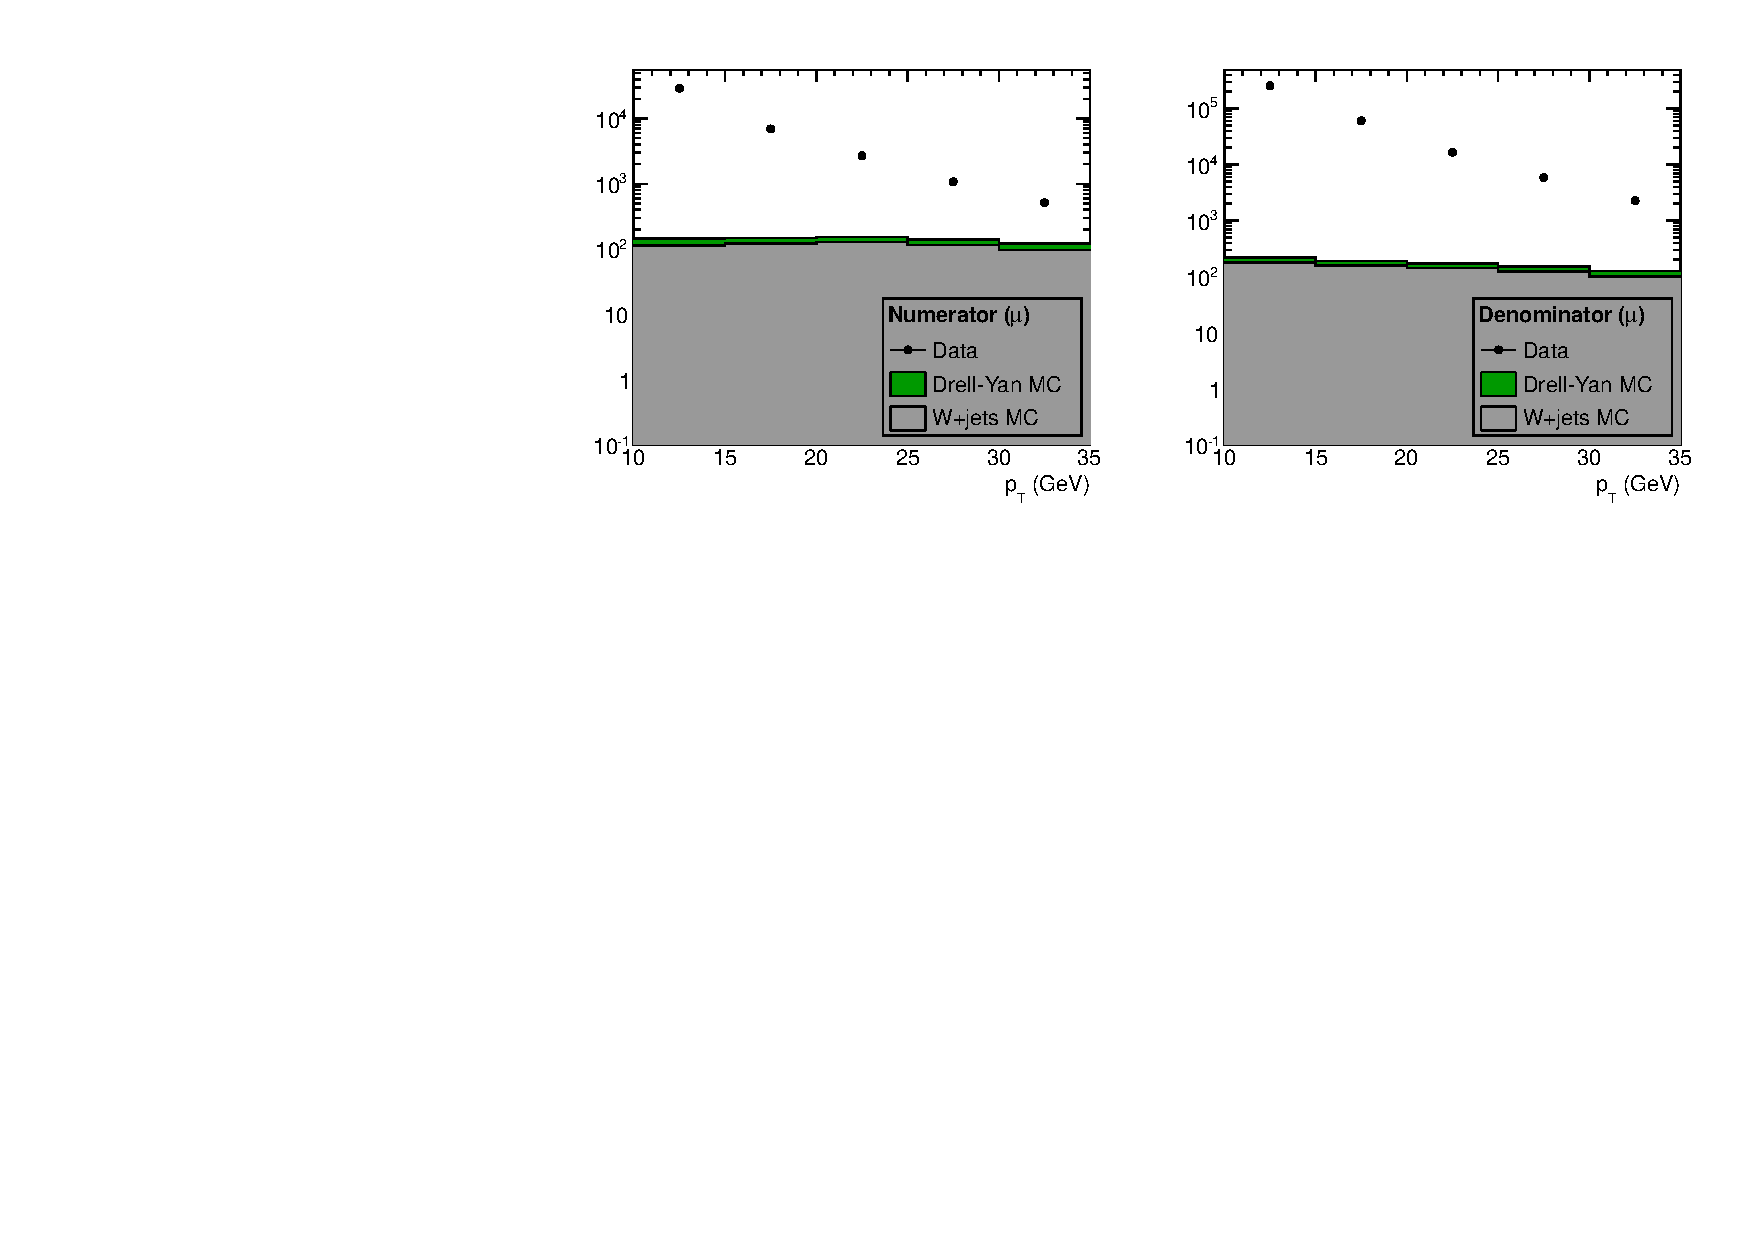
\includegraphics[width=1.00\textwidth]{figures/Num_den_pt_Mu.pdf}  \\
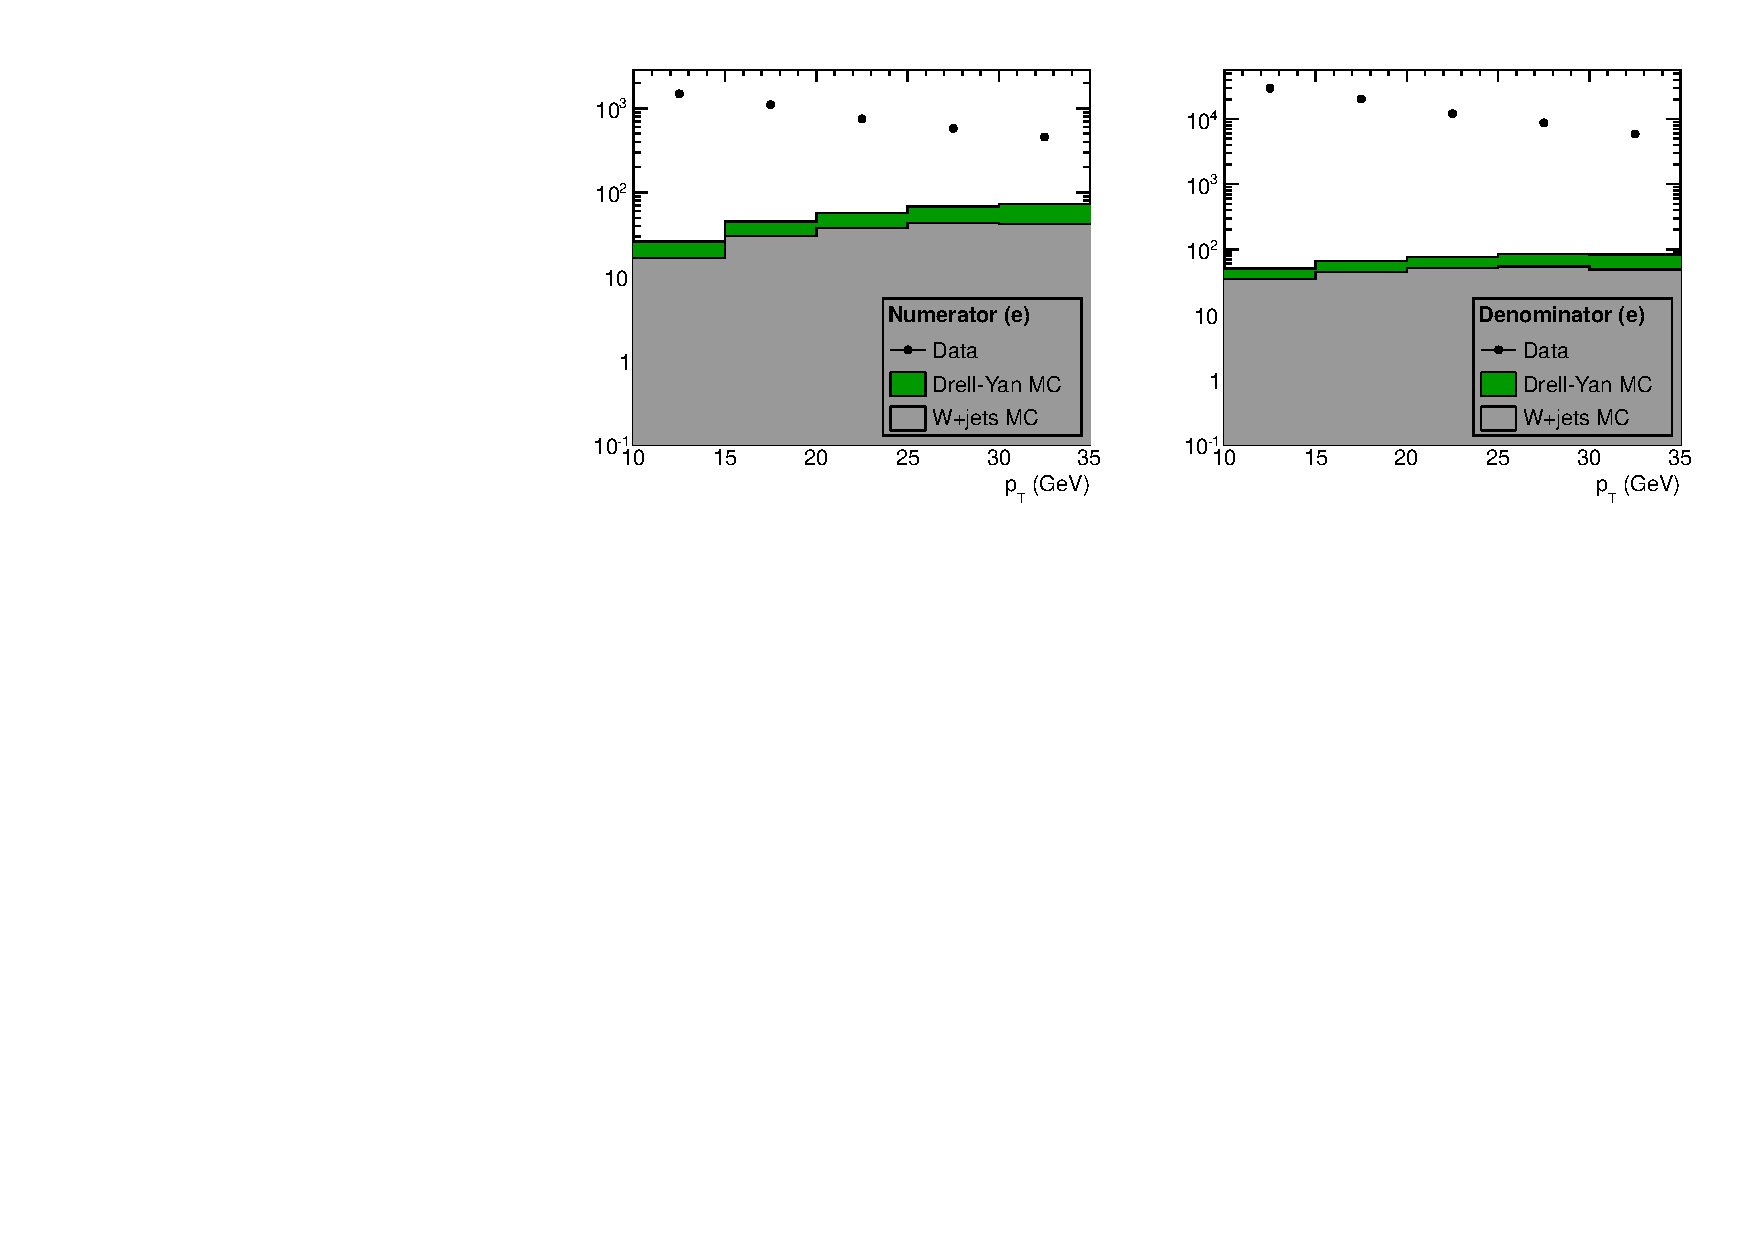
\includegraphics[width=1.00\textwidth]{figures/Num_den_pt_Ele.pdf}
\end{tabular} 
\caption{The \pt\ of denominator(left) and numerator(right) of 
muon FO(top) and electron FO(bottom). The black dots represent 
data and solid histograms represent contributions from Drell-Yan(green) 
and W+jets(grey). It is obvious 
that the contribution from EWK processes is quite large at high FO \pt\ 
and FR would be higher if EWK contribution were not subtracted
because FR of EWK sample is higher than the FR of QCD di-jet sample.  }
\label{fig:Num_Den_pt_EWK} 
\end{figure} 
Figure~\ref{fig:Num_Den_pt_EWK} shows the \pt\ distributions of denominator and the 
numerator of electron and muon FO. The data is shown with black dots and 
the EWK contributions from \dyll\ and \Wjets\ are shown in green 
and grey, respectively. At higher FO \pt\ the EWK contribution 
is larger. Because FR is higher in \Wjets\ events than the QCD di-jet 
events, if EWK contribution were not subtracted, the FR would be 
measured higher than it should be. The subtaction of EWK contribution 
reduces FR in the last \pt\ bins by up to 30 \%.

The lepton fakes originate from a parton and the fake rates have strong 
correlation with the \pt\ of the parton from which a fake lepton originates.
So, it is very important to use the same kinematic region used to measure FR 
is similar with the region where the FR is applied. The best handle is the 
\pt\ of the pre-genetor parton, but this information is not available in data.   
We use the \pt\ of the jet which is separated by $\Delta \textrm{R(FO, leading jet)} > 1.0$.  
Given that the FR is measured with the sample dominated by QCD di-jet events, 
the FO and the leading jet tend to be back-to-back in the $r-\phi$ plane.
There for by gauging the \pt\ of the away jet, we can gauge the \pt\ 
of the pre-genetor of the FO. Ideally this works, but reality is more 
complicated because the \pt\ of the away jet does not necessarily represent 
the \pt\ of the pre-genetor of the FO. The away jet \pt\ can be mis-measured 
and the direction of the jet can be off back-to-back direction.  
Therefore, it is not straightforward to decide the \pt\ of the away jet. 

We use the same-sign events to make sure that we select the 
relevant kinematic range of the pre-genetor for the \Wjets\ sample. 
These events are dominated by \Wjets\ and $\wgamma(^*)$. Since we control $\wgamma(^*)$
relatively well, we can use these events to confirm that the measured 
FR predicts the data correctly. 
But, even though the prediction is consistent with observation, 
we can not conclusively claim that the measured FR is correct 
because the composition of fakes can be different in the SS and OS events. 
For example, same-sign events can not come from W+q events, 
which result in an opposite-sign lepton pair\footnote{If W has (+1) charge, 
q has (-1/3) charge which makes up a (-1) charge meson, and it subsequently decays 
to a (-) charge lepton. The ratio of OS to SS measured in \Wjets\ MC 
is 6:4}. Therefore, the result using SS events can 
give a guess, and we can not conclusively decide the away jet \pt. 
Using away jet \pt\ thresholds, 35~\GeV\ for electrons and 
30~\GeV\ for muons, the expected SS events in the 0-jet bin 
is $794\pm18(stat.)$ while the number of observed data events is 752. 
\begin{figure}[htp] 
\centering 
\begin{tabular}{c} 
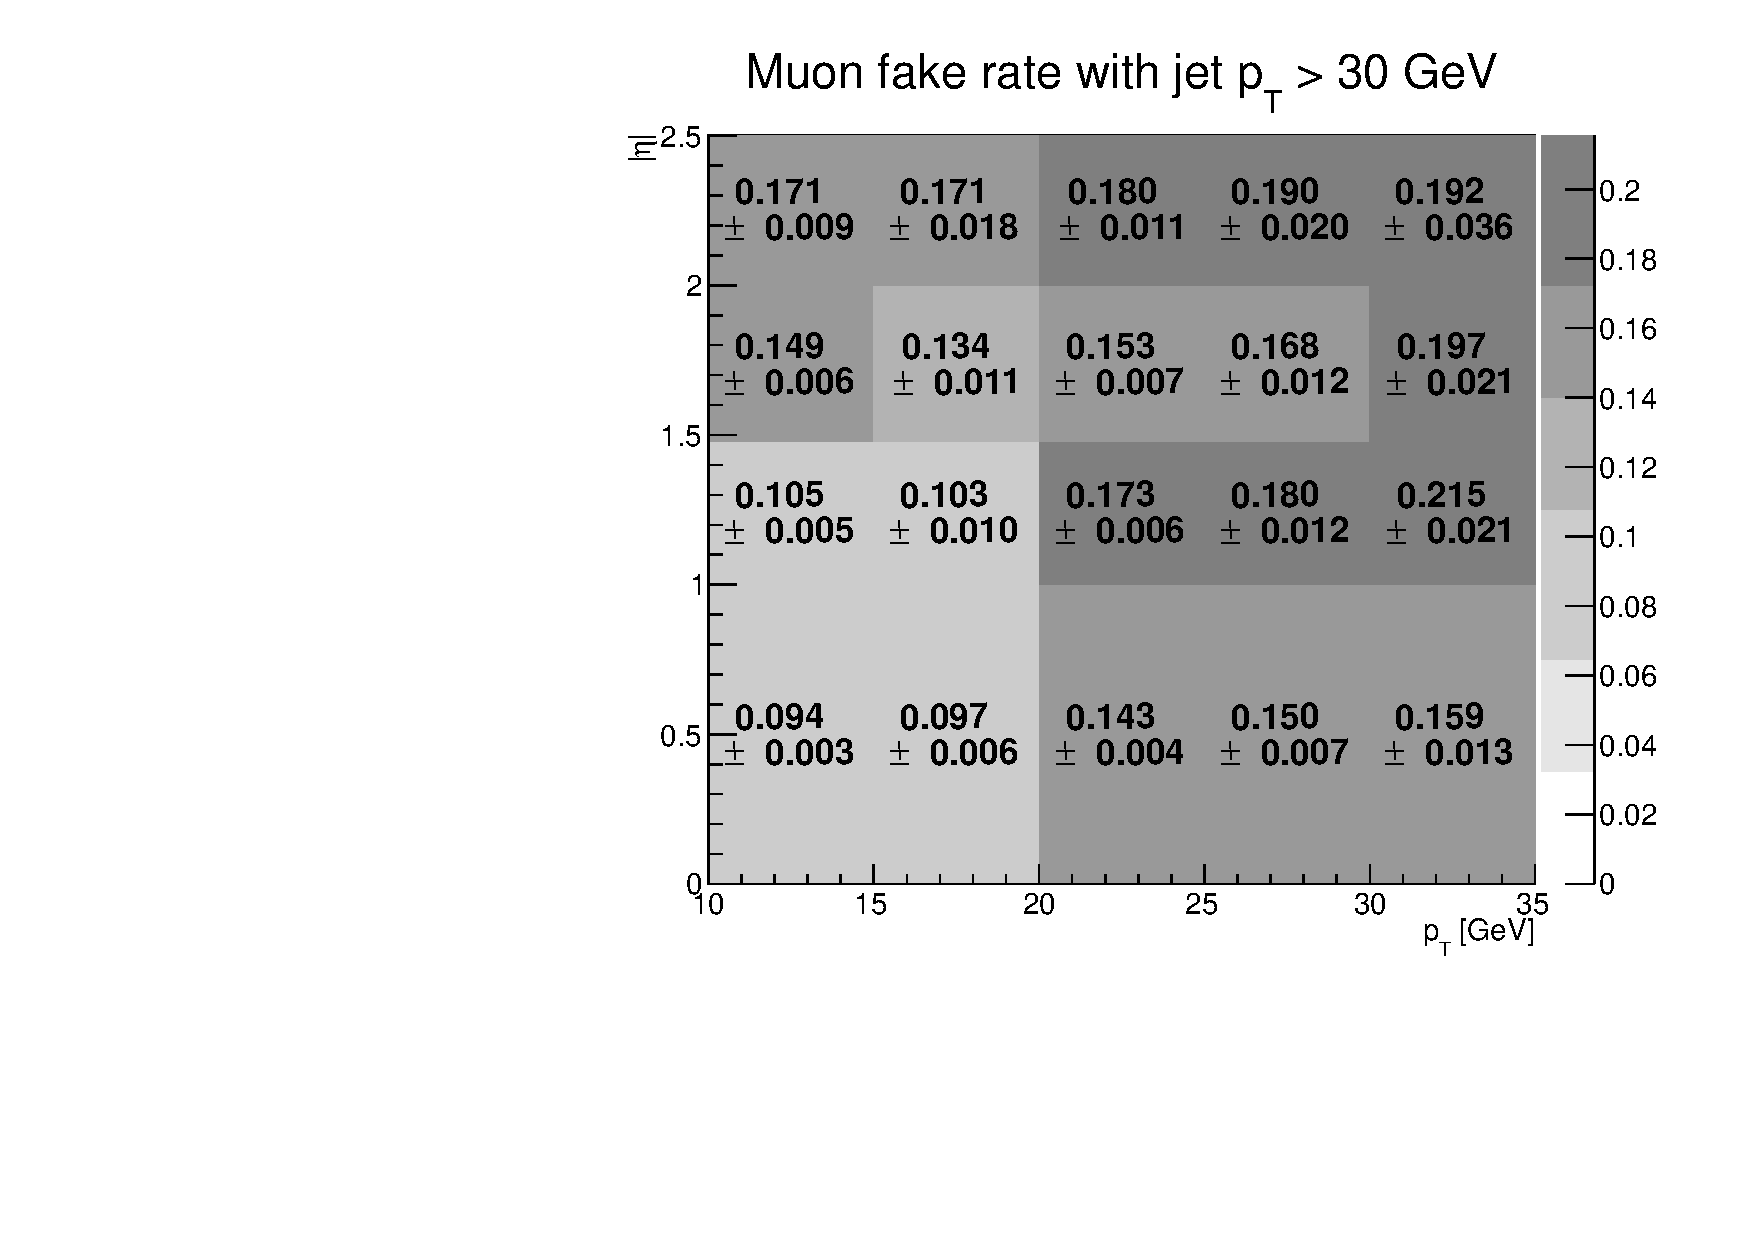
\includegraphics[width=0.75\textwidth]{figures/2DFR_Muon_jet30.pdf} \\
\\
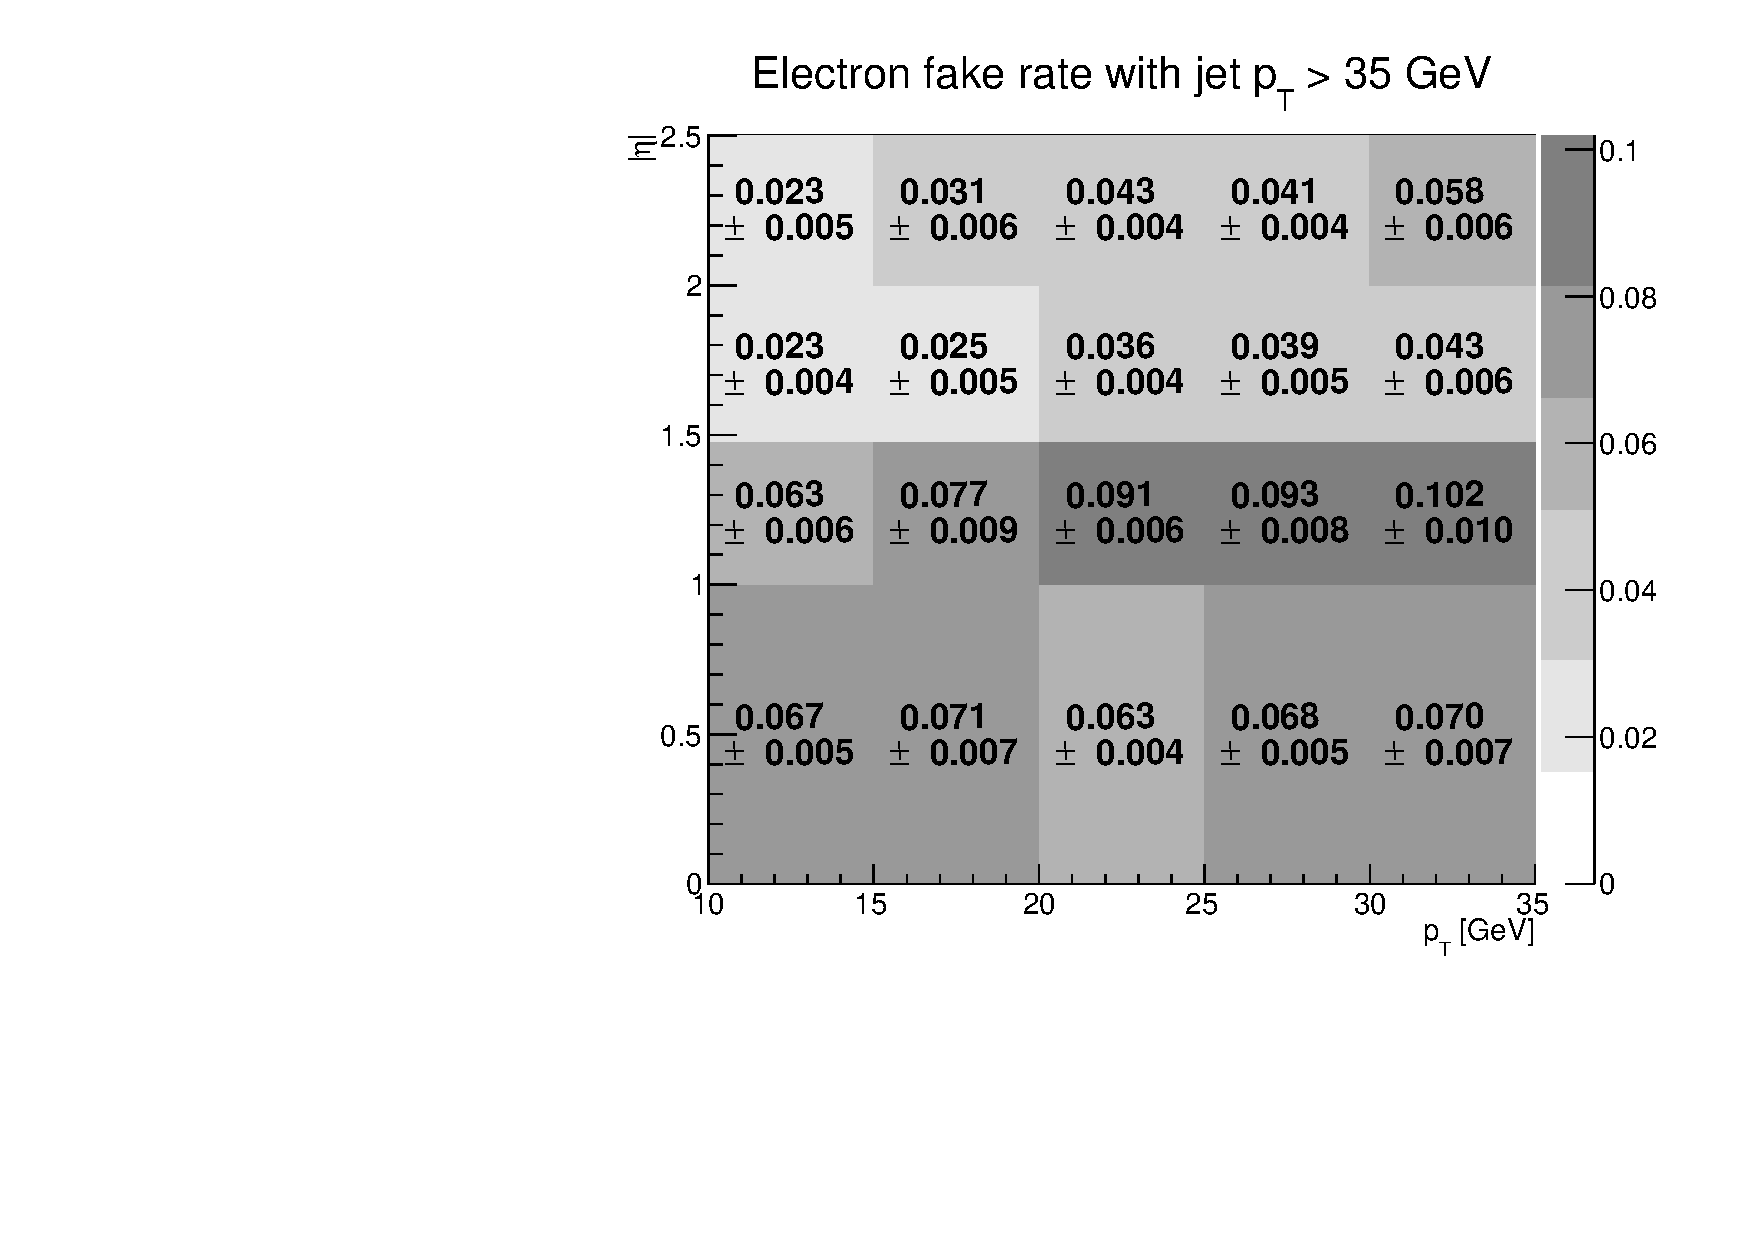
\includegraphics[width=0.75\textwidth]{figures/2DFR_Electron_jet35.pdf}
\end{tabular} 
\caption{Top shows muon fake rate as a function of FO \pt\ and \Eta, 
measured with the away jet $\pt>30~\GeV$.  
Bottom shows electron fake rate as a function of FO \pt\ and \Eta,
measured with the away jet $\pt>35~\GeV$.
The errors are statistics only.
}
\label{fig:2DFR} 
\end{figure} 


\subsubsection{Application of fake rate}

The measured FR as a function of FO \pt\ and \Eta\ is used to predict the 
contribution of \Wjets\ in the signal region. In data we first select events 
in which one lepton passes the full lepton selection while the other lepton 
passes the FO selection but the full selection (Tight+Loose sample). 
The contribution from other 
background processes are subtracted in order to get the pure \Wjets\ sample. 
\begin{figure}[htp] 
\centering 
\begin{tabular}{c} 
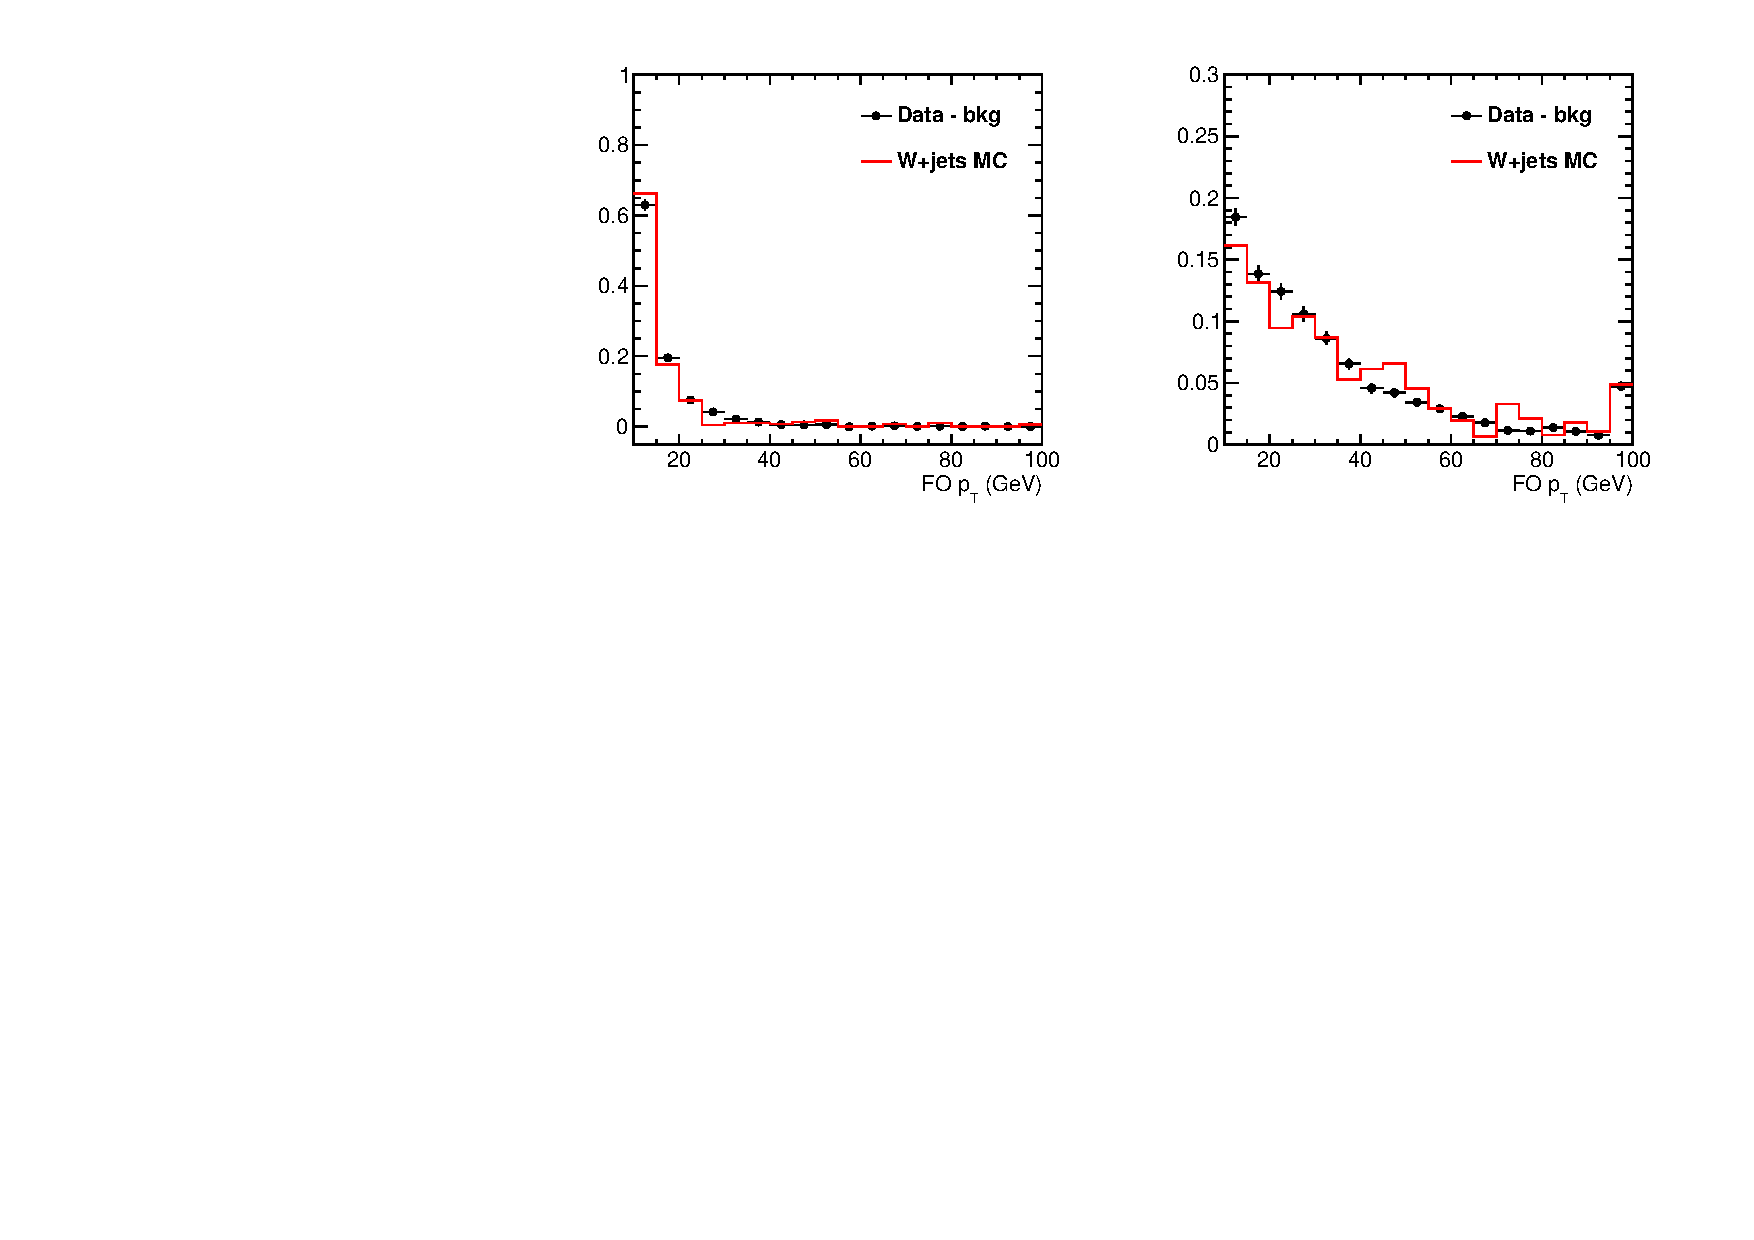
\includegraphics[width=1.00\textwidth]{figures/FOpT_0j_of.pdf} 
\end{tabular} 
\caption{The \pt\ of muon FO (left)and electron FO(right). 
Plots are normalized to the unit area. 
On each plot, the shape of data after subtracting other backgrounds,
and that of \Wjets\ MC are compared. 
They have consistent shapes giving confidence that the selected data sample 
is dominated by \Wjets\ process. } 
\label{fig:FOpT} 
\end{figure} 
Figure~\ref{fig:FOpT} shows the \pt\ distribution of muon and electron FO
on left and right, respectively. The plots are normalized to the unit area.
The data with other backgrounds subtracted amd the \Wjets\ MC show good
agreement in shape giving confidence that the selected data sample
is dominated by \Wjets\ process. Now we use the measured FR as a weight to the 
Tight+Loose sample in the following way.   
\begin{eqnarray} 
N_{\Wjets}^{\textrm{prediction}} 
= \sum_i^{N_{\textrm{Tight+Loose}}} \frac{\textrm{FR}({\pt}_i, \eta_i)}{1 - \textrm{FR}({\pt}_i, \eta_i)}    
\end{eqnarray} 
where $N_{\Wjets}^{\textrm{prediction}}$ is the prediction of \Wjets\ background 
in the signal region, $N_{\textrm{Tight+Loose}}$ is the number of Tight+Loose events
and ${\pt}_i$ and $\eta_i$ are the \pt\ and \Eta\ of the Loose lepton in the $i^{th}$ 
Tight+Loose event.

\subsubsection{Systematics}
%
\begin{figure}[htp] 
\centering 
\begin{tabular}{c} 
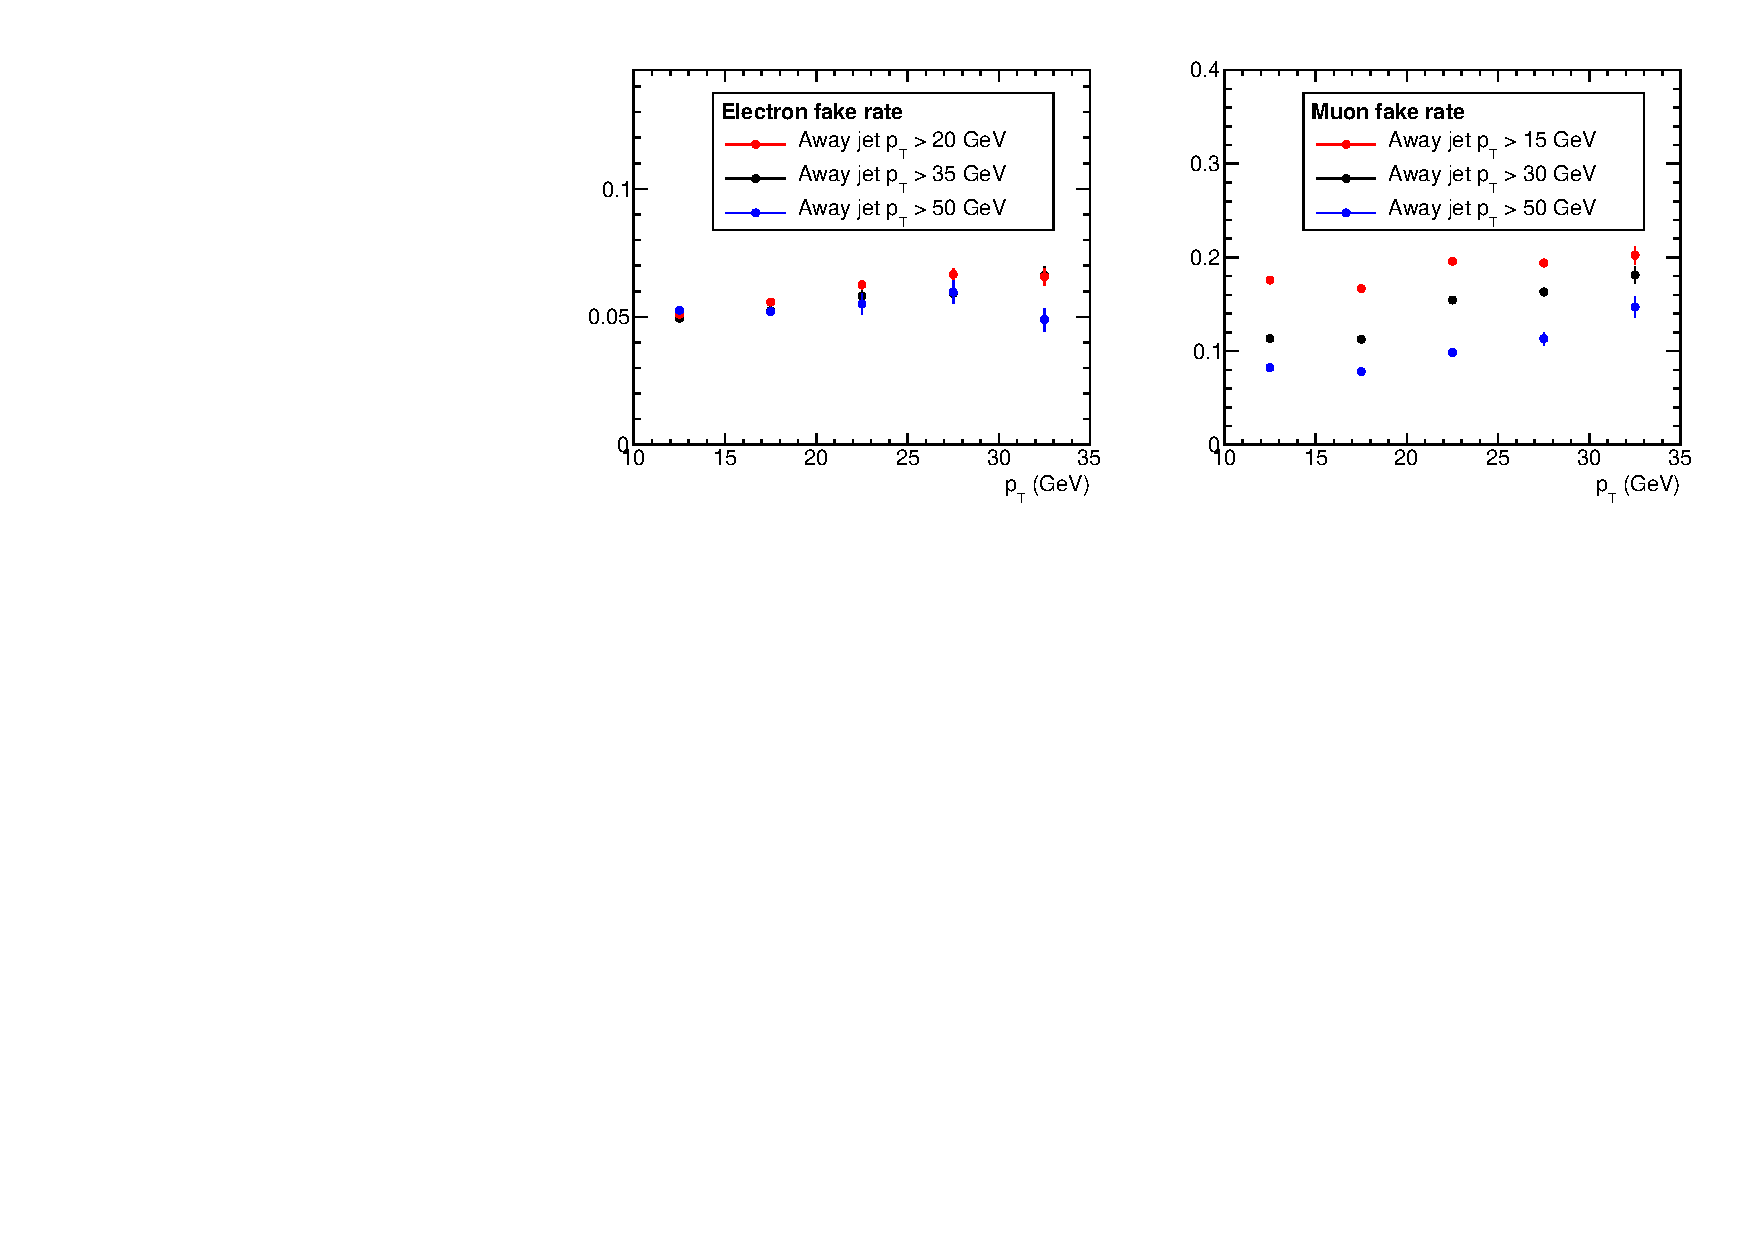
\includegraphics[width=1.0\textwidth]{figures/FR_jetpt_variation.pdf}
\end{tabular} 
\caption{Left plot is the electron fake rates projected on \pt\ for 
different away jet \pt\ thresholds, 20, 35(default) 50~\GeV. 
Right plot is the muon fake rates projected on \pt\ for
different away jet \pt\ thresholds, 15, 30(default) and 50~\GeV.} 
\label{fig:FR_jetpt_variation} 
\end{figure} 
As mentioned before, the away jet \pt\ is a handle for the QCD di-jet events 
to give relevant kinematic range for FO in \Wjets, and it is decided based on the SS events 
result which is not conclusive. We, therefore, assign systematic uncertainty 
to account for our ignorance on the controlling the pre-genetor \pt\ 
by varying the away jet \pt\ threshold
to cover the relevant kinematic range of the \Wjets\ sample.
Fig.~\ref{fig:FR_jetpt_variation} shows the dependence of FR on the 
away jet \pt\ thresholds. Left plots shows the dependence of electron 
FR and the right plot shows the dependence of muon FR. 
The alternative away jet \pt\ thresholds are 20~\GeV\ for electrons 
and 15~\GeV\ for muons. The prediction using the alternative \pt\ thresholds
differ by 30 \% compared to the nominal results, and this difference 
is taken as systematic uncertainty. 
% WW level 0-jet 
% Ele : 380 ==> 395 : 5 % up
% Mu  : 415 ==> 638 : 50 % up
In addition, composition of the sample can be different in QCD di-jet sample, 
and \Wjets\ sample. So, we do MC closure test assuming that the parton composition 
is well-modeled by MC. The result shows that the difference between 
prediction and observation is $\sim$ 20 \% for both electrons and muons.
The two systematic uncertainties are combined in quadrature, resulting 
36 \% total systematic uncertainty for both electrons and muons. 

%%%%%%%%%%%%%%%%%%%%%%%%%%
\section{ \topbkg }

The backgrounds induced by top quarks come from \topbkg\ processes where 
the W's decayed from top quarks decay leptonically. These processes 
result in two isolated leptons with considerable \met, which is 
same as the signature of signal events, and b-tagged jets which
is used to suppress this background. However, in case the b-jet 
goes out of the tracker coverage or it is not tagged as a b-jet, 
these events can fall survive the signal selection. We use 
data-driven methods applied to 0-jet and 1-jet separately.

The top background is estimated after WW selection and a common 
data/MC scale factor for \topbkg\ is calculated in 0-jet and 1-jet 
categories. Then, MC is normalized with the measured scale factor 
to be used for the shape-based analysis. The basic idea of the 
top estimation is to reweight the Top-tagged region using the 
top-tagging efficiency obtained from an indepdent sample. This 
can be expressed as the following formula, 
\begin{eqnarray} 
N_\textrm{top-veto} 
= 
N_{\textrm{top-tagged}} \times
\frac{1 - \epsilon_{top-tagging}}{\epsilon_{top-tagging}}   
\end{eqnarray} 
where $N_\textrm{top-veto}$ is the prediction for top-vetoed events 
in the signal region, $N_{\textrm{top-tagged}}$ is the number of 
top-tagged events which can be obtained by inverting the top-veto requirement, 
and $\epsilon_{top-tagging}$ is the top-tagging efficiency 
measured in an independent sample. The top-taggeing efficiency 
is measured in a different way in the 0-jet and 1-jet categories.

\begin{table}[!h]
\begin{center}
\small
\begin{tabular} {|c|c|c|c|c|}
\hline
jet bin & top veto & top tag & $\epsilon_{tag}$ denominator & $\epsilon_{tag}$ numerator \\ 
\hline
0       & no soft muon,      & either a soft muon  & 1-jet bin, leading & denom. + \\
        & no low \pt\ b-jets & or a low \pt\ b-jet & jet is btagged     & top tag  \\
\hline
1       & no soft muon,           & leading jet  & 2-jet bin, sub-leading & denom. + \\
        & no low/high \pt\ b-jets & is b-tagged  & jet is btagged         & top tag  \\
\hline
\end{tabular}
\caption{Summary of selection and control region definitions used 
in top estimation in the different jet bin.}
\label{tab:topbkgest}
\end{center}
\end{table}

\subsubsection{0-jet category method}

We start with measuring ``per-leg" tagging efficiency.
In the \ttbar\ events, there are two b-quarks in the final states, 
so we can explore the second b-quark after requireing that the first b-quark be tagged. 
A caveat is that the \tw\ contribution should be subtracted because
those events have only one b-quark in the final state, and the second 
jet is from FSR or ISR regardless of jet flavor. 
Some of the FSR or ISR jets can be b-tagged as well and this 
makes \tw\ indistinguishable from \ttbar. Therefore, this should 
be accounted for when calculating top-tagging efficiency. 

The denominator is defined by requiring exactly one b-tagged jet with $\pt>30~\GeV$. 
This requirement to select a sample dominated by \topbkg.  
Of the selected events, a subset of events containing at least one b-tagged jet
with $10<\pt<30~\GeV$ or one soft-muon becomes numerator. 
The ratio of the yields in numberator to denominator after subtracting contributions 
from other backgrounds as well as \tw\ is the top-tagging efficiency for one leg, 
$\epsilon_{per-leg}^{data}$. 

The ``per-event" top-tagging efficiency is then calculated by the following equation, 
\begin{eqnarray} 
\label{eq:TopTagEff0jet}
\epsilon_{\textrm{top-tag, per-event}}^{data} 
= 
\begin{array}{ccc} \multicolumn{2}{c}{\displaystyle 
\left(1-\left(1-\epsilon_{per-leg}^{data}\right)^2\right) 
\left(f_{t\bar{t}}^{MC} + x\left(1-f_{t\bar{t}}^{MC}\right) \right)
} & \\ & \multicolumn{2}{c}{\hspace{5cm} \displaystyle
+ \left(1-f_{t\bar{t}}^{MC}\right)\left(1-x\right)\epsilon_{per-leg}^{data}
} \end{array}   
\end{eqnarray} 
where the first term corresponds to the tagging efficiency for the events with 
two taggable legs, and the second term corresponds to the tagging efficiency for 
the events with one taggable jet. 
The $\epsilon_{\textrm{top-tag, per-event}}^{data}$ is the per-event top-tagging efficiency. 
The $f_{t\bar{t}}^{MC}$ is the fraction of \ttbar\ events with respect to the 
\ttbar+\tw\ events measured using MC at WW level requiring no jets. 
The $x$ is the fraction of events that contain two taggable legs in \tw\ events. 
It approximately corresponds to the $\epsilon_{per-leg}$ measured in \tw\ MC.  

Finally, the control region in data is defined by inverting the top-veto requirement, 
\textit{i.e.}, requiring soft-muon or b-tagged jets with $10<\pt<30~\GeV$.
The contributions from other backgrounds are subtracted so that the 
measured top-tagging efficiency is applied to only \topbkg\ events. 
The left plot in fig.~\ref{fig:TCHE_topCR} shows the level agreement between 
data and MC in the top control region for 0-jet category.  
They show good agreement and we conclude that the data subtracted by other backgrounds 
will give \topbkg\ events with high purity. 
The prediction of \topbkg\ events in the signal region is calculated by 
\begin{eqnarray} 
\label{eq:topExtrapolation0jet}
N^{top}_{\textrm{WW region}}
%&=&  
%N_{top-tag}^{\textrm{top CR, \topbkg}} \times
%\frac{1-\epsilon_{\textrm{top-tag, per-event}}^{\textrm{data}}}
%     {\epsilon_{\textrm{top-tag, per-event}}^{\textrm{data}}} \\ 
&=&   
(N_{top-tag}^{\textrm{data}}-N_{top-tag}^{\textrm{other bkg}}) \times
\frac{1-\epsilon_{\textrm{top-tag, per-event}}^{\textrm{data}}}
     {\epsilon_{\textrm{top-tag, per-event}}^{\textrm{data}}}.  
\end{eqnarray} 
where $N_{top-tag}^{\textrm{data}}$ is the data count in the top CR 
and $N_{top-tag}^{\textrm{other bkg}}$ is the contribution from other 
background process in the top CR.

The systematic uncertainty to the top estimation in the 0-jet category 
is dominated by the uncertainty to the parameter $x$. The uncertainties
for the \ttbar\ and \tw\ cross sections are about 7 \% and 15 \%~\cite{Kidonakis:2012rm}, 
and these make the uncertainty of $x$ 17\%. 

\subsubsection{1-jet category method}

The method for measuring top-tagging efficiency for 1-jet category is 
based on the fact the b-tagging efficiency of the most energetic jet 
in 1-jet and 2-jet categories is approximatley same. The efficiencies 
measured in \ttbar\ MC after WW selection is 66 \% and 67 \% in 1-jet 
and 2-jet categories, respectively. Therefore, we measure the b-tagging 
efficiency of the most energetic jet in the the events containing 2-jets
and apply this to the control region in the 1-jet category.  
The definition of control region is different from an inversion of 
the top-veto requirement in this case because the b-tagging efficiency 
is correlated with existence of soft-muons in the jet. 
So, the control region is defined without soft-muon requirement, 
and this definition is consistently applied for the top-tagged region, 
top-vetoed region and the top-tagging efficiency measurement.
The right plot in fig.~\ref{fig:TCHE_topCR} shows the level agreement between 
data and MC in the top control region for 1-jet category.  
They show good agreement and we conclude that the data subtracted by other backgrounds 
will give \topbkg\ events with high purity. 

Then, the top contribution in WW region is calculated using the measured
top-tagging efficiency($\epsilon_{\textrm{top-tag, per-event}}^{\textrm{data}}$) 
and the number of events in the top CR($N_{top-tag}^{\textrm{data}}
-N_{top-tag}^{\textrm{other bkg}}$) as shown in the eq.~\ref{eq:topExtrapolation0jet}.

\begin{figure}[htp] 
\centering 
\begin{tabular}{c} 
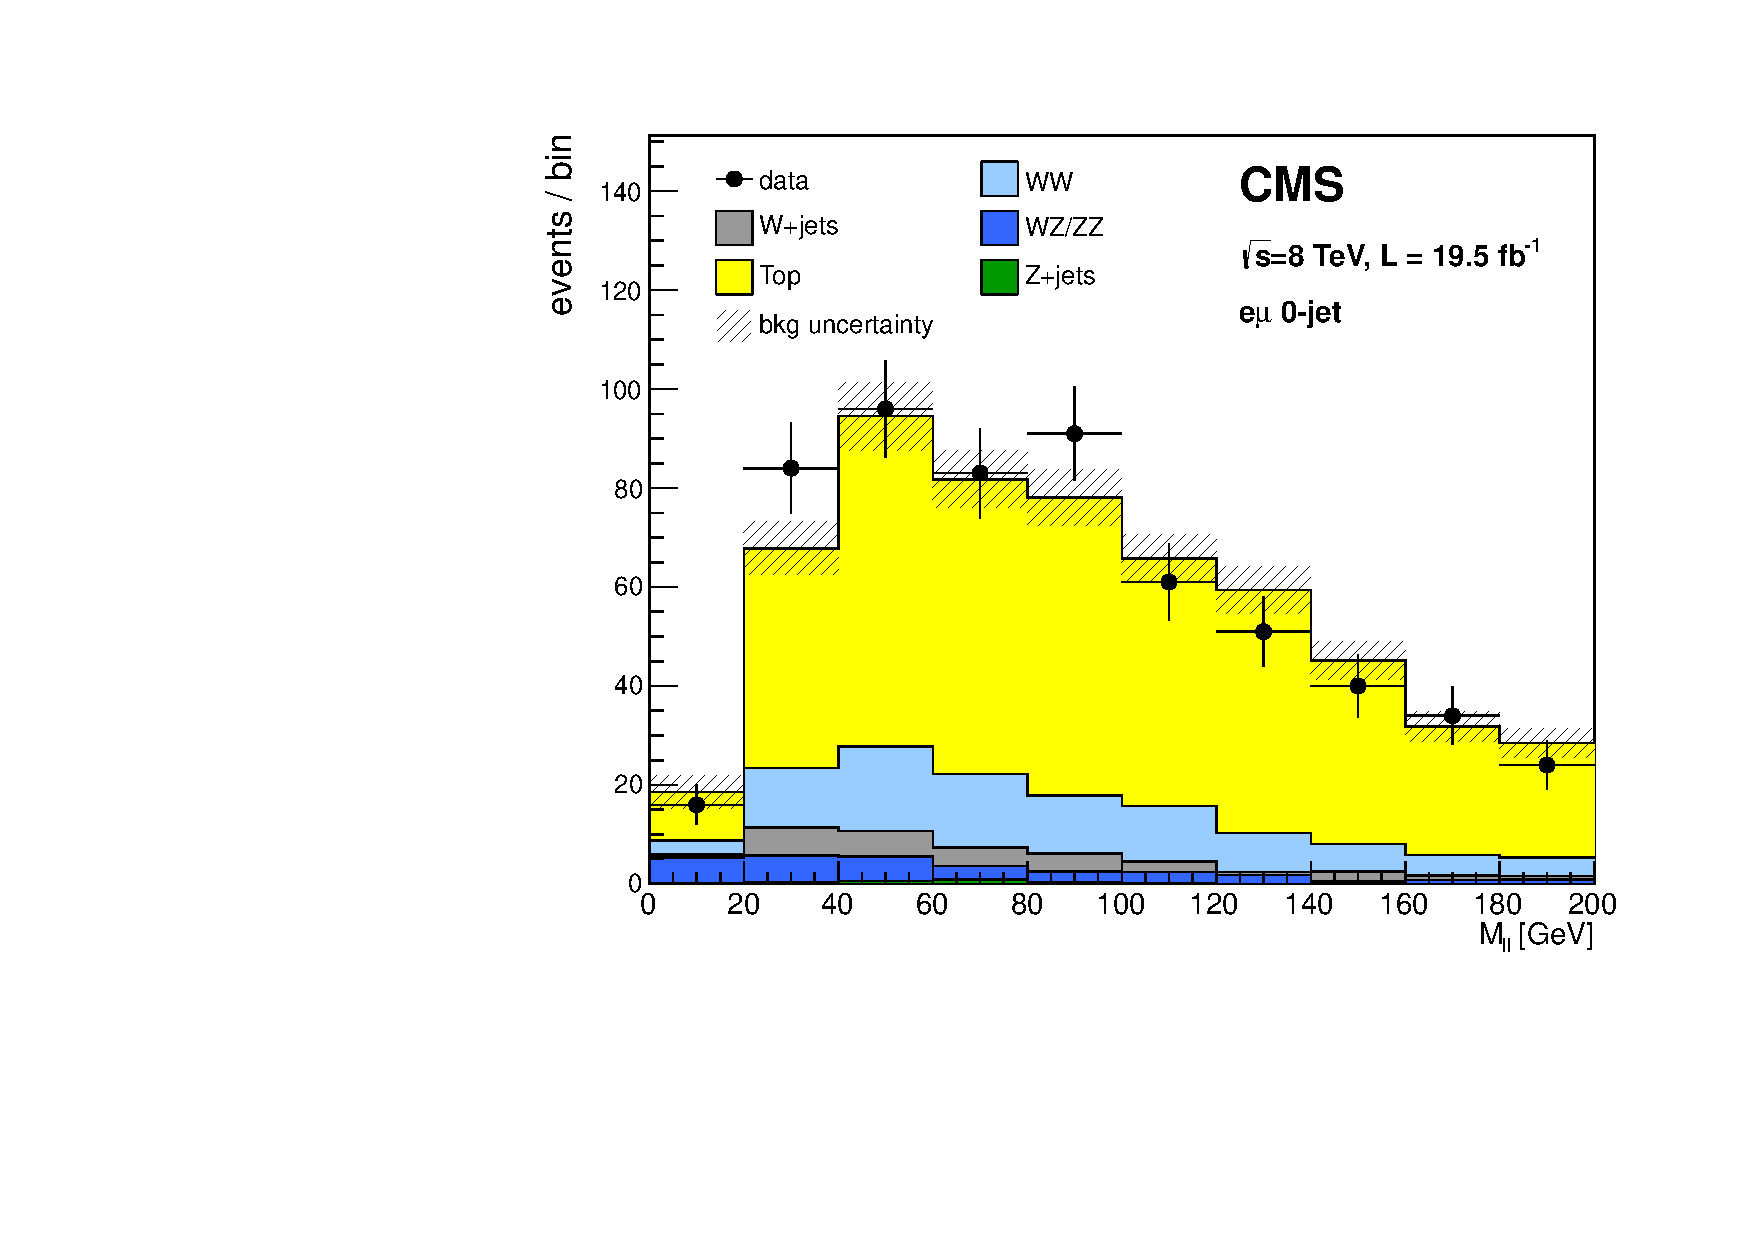
\includegraphics[width=0.5\textwidth]{figures/topcontrol_mll_of_0j.pdf}
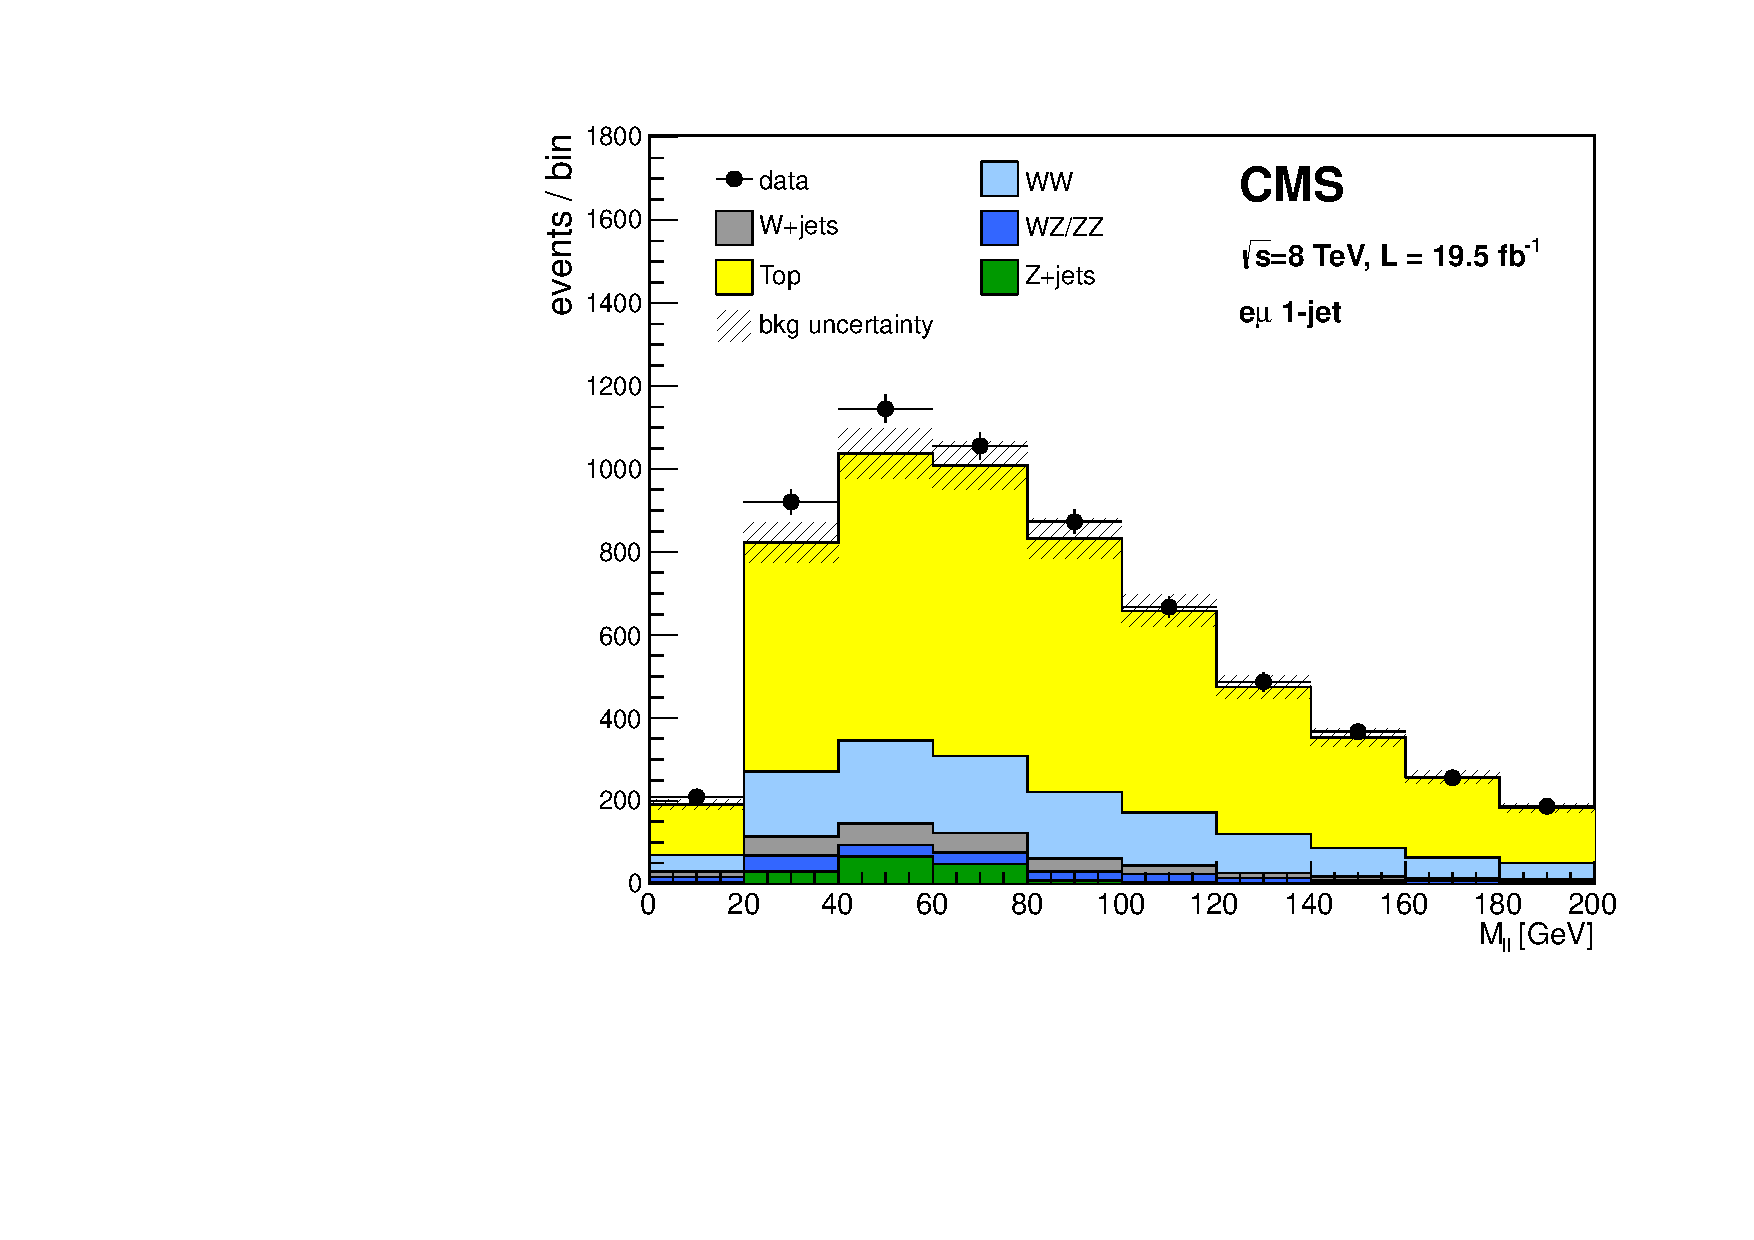
\includegraphics[width=0.5\textwidth]{figures/topcontrol_mll_of_1j.pdf} 
\\
\includegraphics[width=0.5\textwidth]{figures/topcontrol_mt_of_0j.pdf}
\includegraphics[width=0.5\textwidth]{figures/topcontrol_mt_of_1j.pdf} 
\\
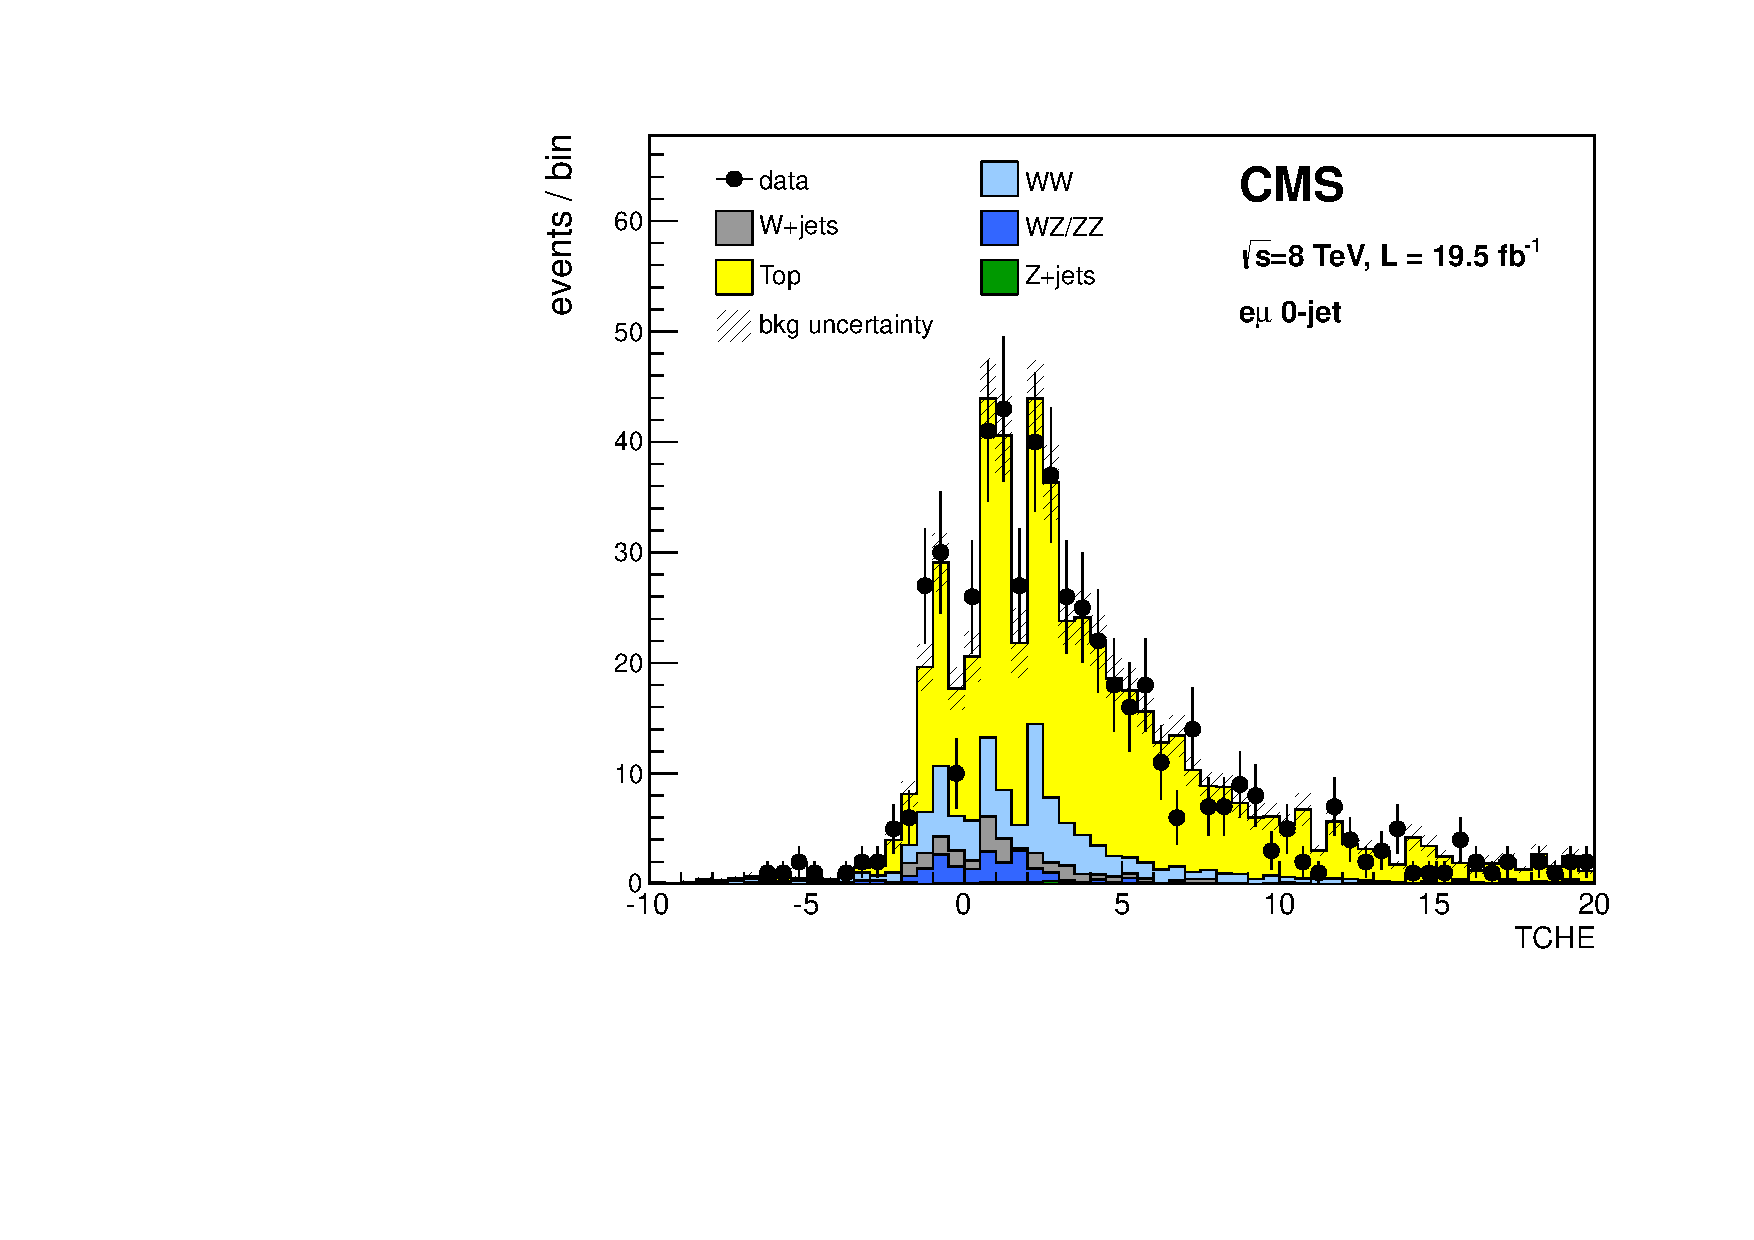
\includegraphics[width=0.5\textwidth]{figures/topcontrol_tche_of_0j.pdf}
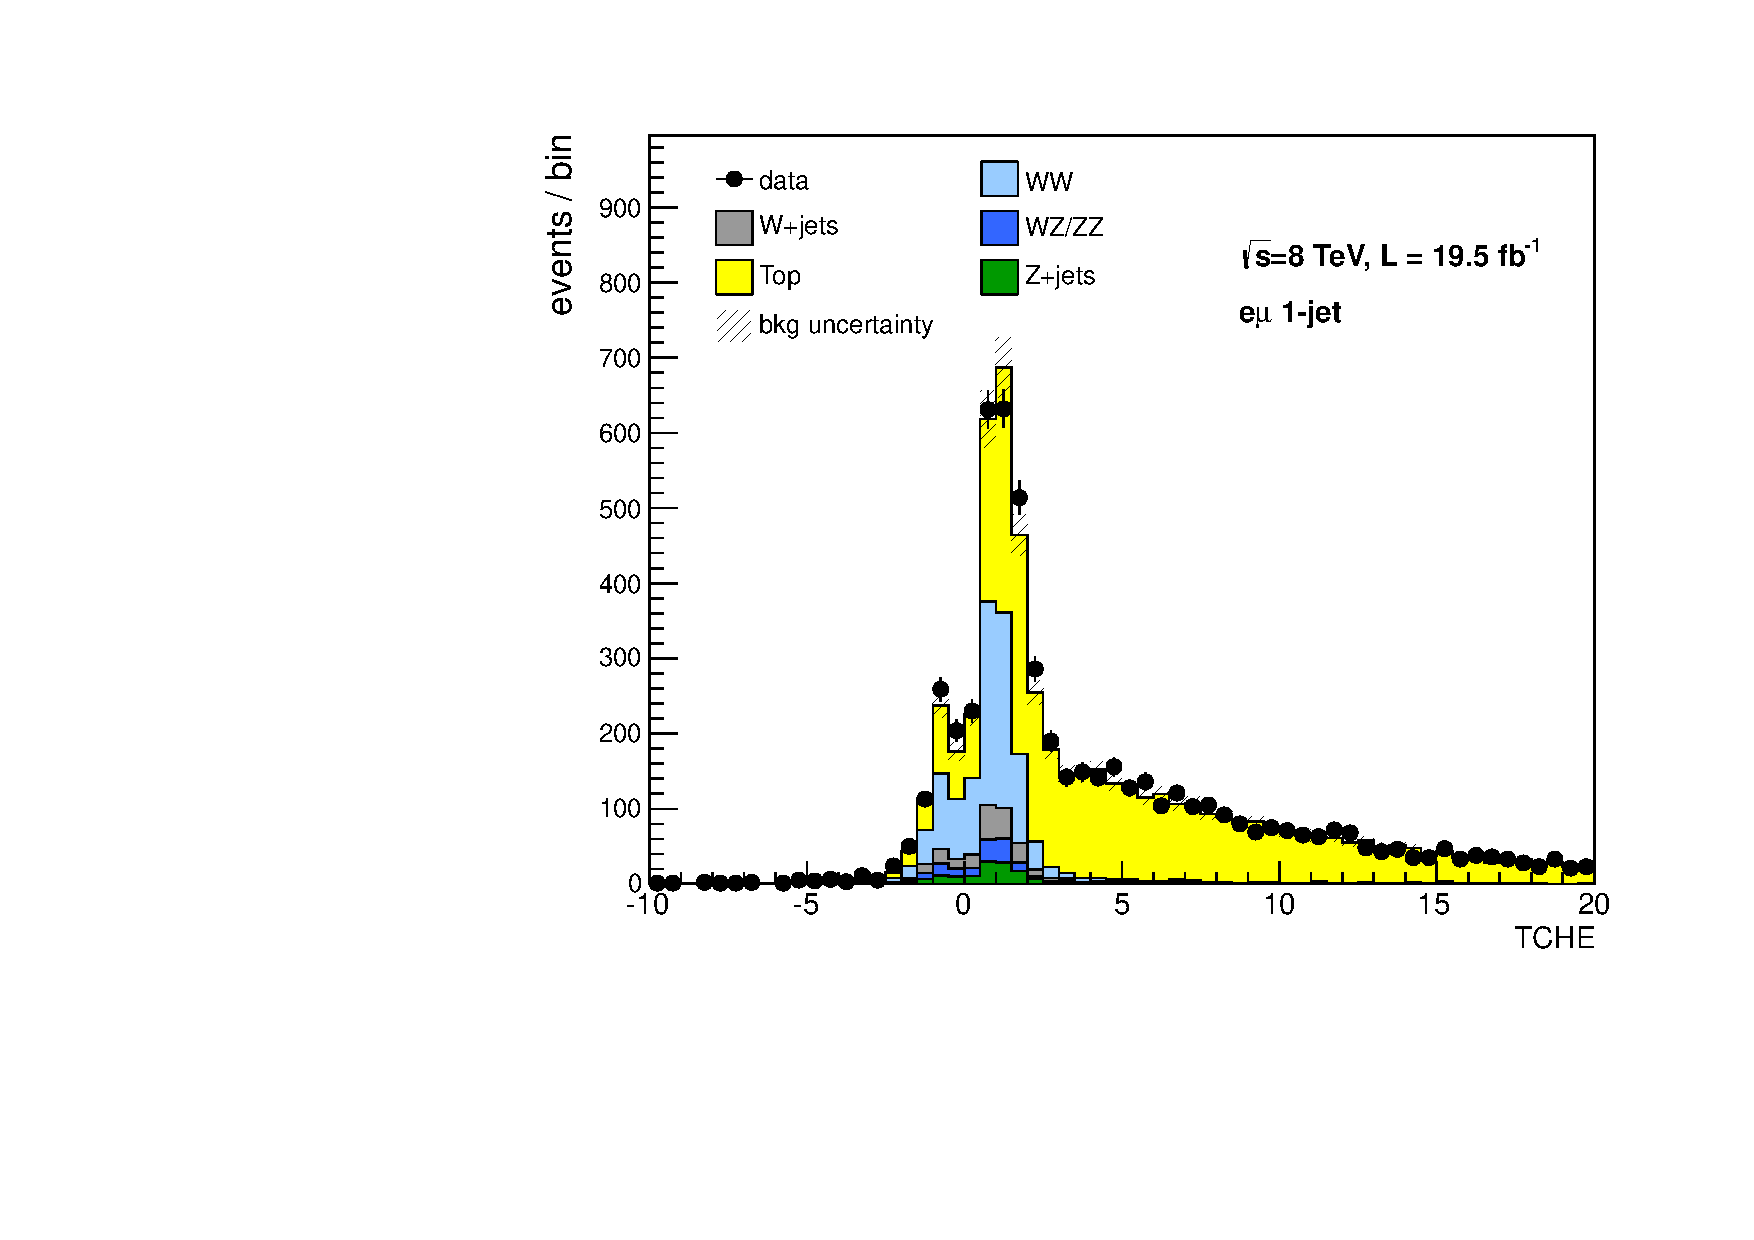
\includegraphics[width=0.5\textwidth]{figures/topcontrol_tche_of_1j.pdf} 
\end{tabular} 
\caption{Distribution of b-tagging discriminator for most energetic jet($\pt>10~\GeV$) 
in the event in the 0-jet(left) and 1-jet(right) top control regions
where top-tagging efficiency is measured. The agreement between data and MC is good, 
and it shows good control of \topbkg\ in the data.} 
\label{fig:TCHE_topCR} 
\end{figure} 

The systematic uncertainty to the top estimation in the 1-jet category 
is dominated by data statistics in the control region which accounts for 
about 2\%.     

\subsubsection{Result}

Tab.~\ref{tab:ttbar_est} show the result of data-driven estimation for \topbkg. 
The data/MC scale factors are consistent to unity in both 0-jet and 1-jet categories. 
The uncertainty is large in the 0-jet category due to the large cross section uncertainty 
of the \tw\ process. The calculated scale factors are applied to the MC counts 
in the signal region.

\begin{table}[ht!]
\begin{center}
\begin{tabular}{c c c}
\hline
                             Sample     & 0-jet                   & 1-jet               \\
\hline
Estimated \topbkg events in simulation  & 720.5 $\pm$   4.3 & 2151.3 $\pm$  13.9        \\
Tagging efficiency     (\%)             & 49.3 $\pm$  4.3   & 64.8 $\pm$  0.5           \\ 
Data events in control region           & 1034              & 4847                      \\ 
Background events in control region     & 292.6 $\pm$  43.9 & 255.5 $\pm$  51.1         \\ 
\topbkg estimation in data              & 761.4 $\pm$ 146.5 & 2307.9 $\pm$  59.4        \\
Data/simulation scale factor            & 1.06 $\pm$  0.20  & 1.07 $\pm$  0.03          \\
\hline

\hline
\end{tabular}
\caption{Monte Carlo to data scale factor for the top background contribution for $\intlumiEightTeV$. 
In the 1-jet bin, the scale factor is derived in a region that is slightly different from the signal region.}
\label{tab:ttbar_est}
\end{center}
\end{table}

%%%%%%%%%%%%%%%%%%%%%%%%%%
\section{ \ww }
\begin{figure}[htp] 
\centering 
\begin{tabular}{c} 
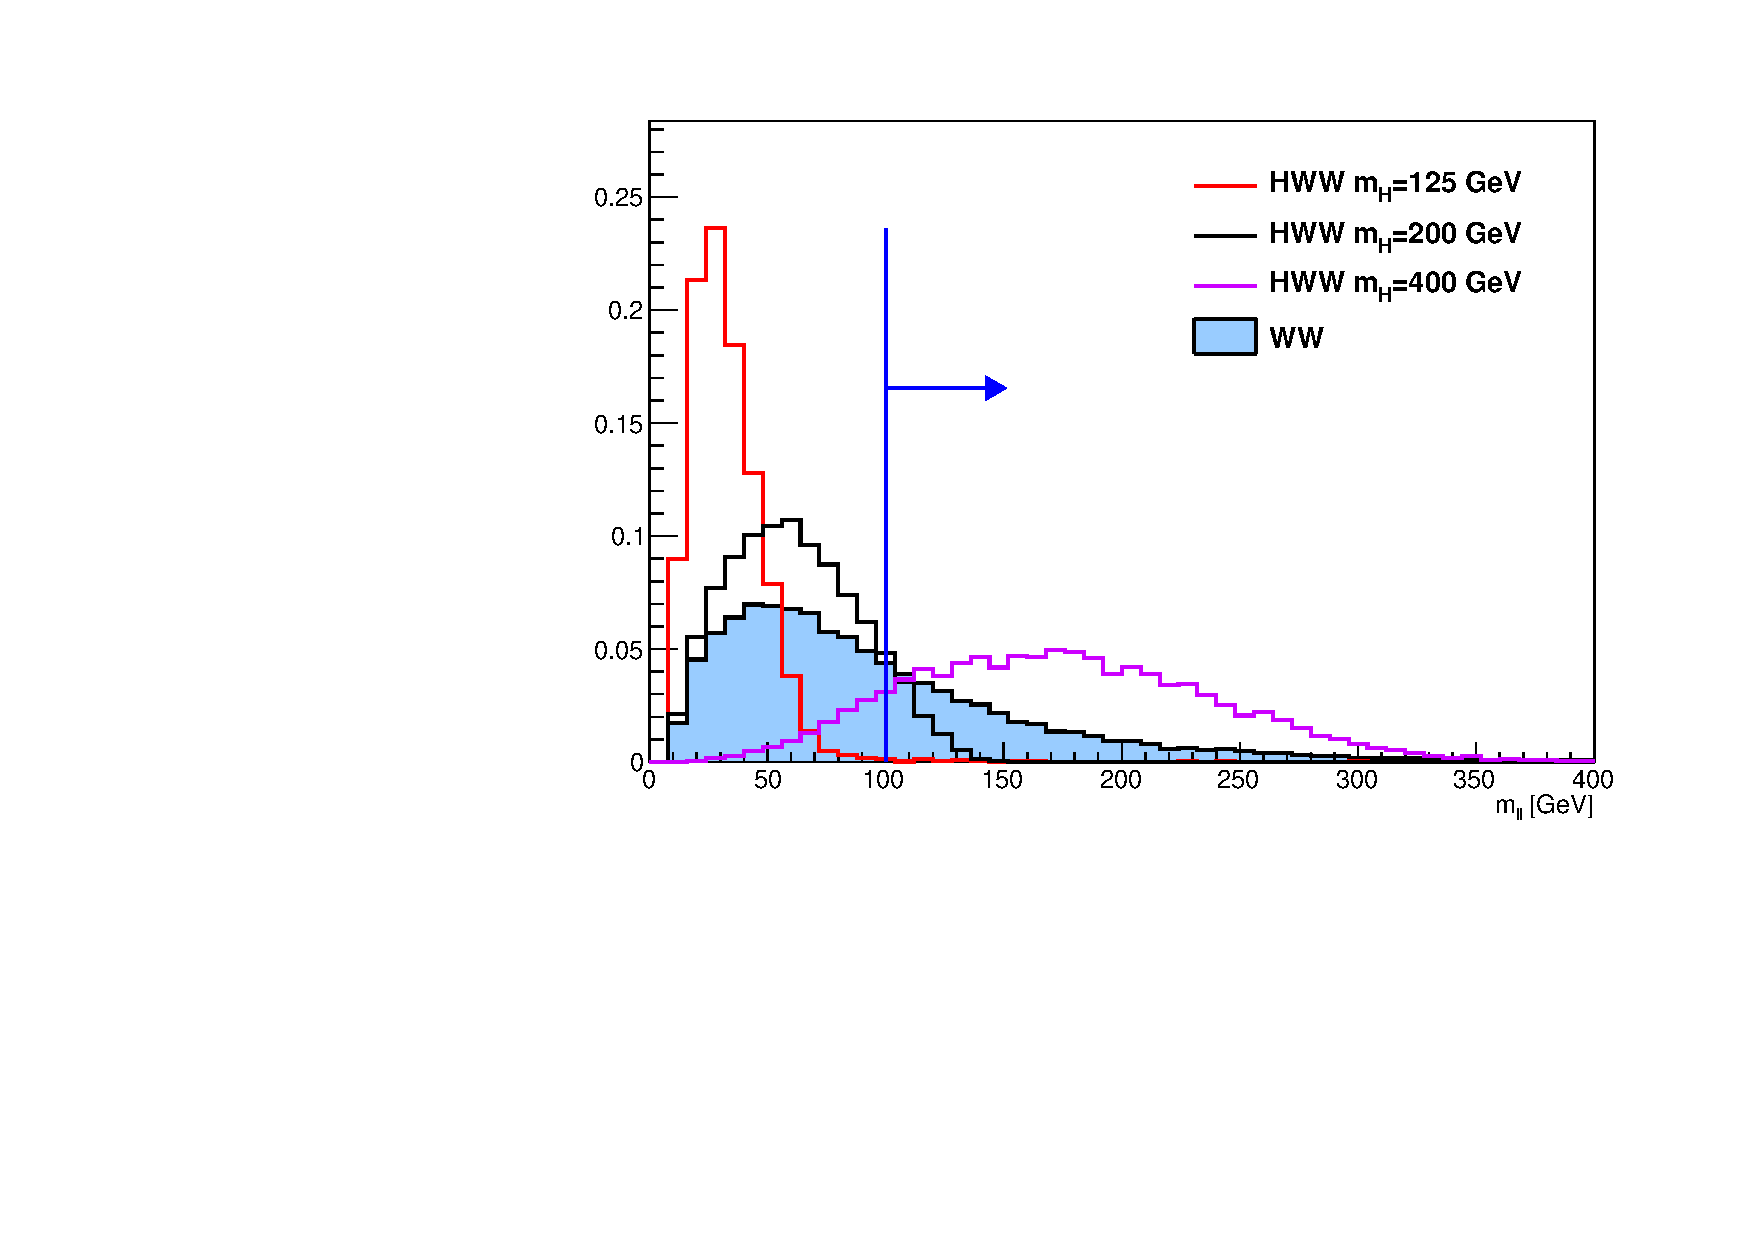
\includegraphics[width=1.0\textwidth]{figures/WW_mll_0j_of.pdf} 
\end{tabular} 
\caption{ \mll\ distributions in 0-jet \DF\ channel for various signal events, 
\mHi=125, 200 and 400~\GeV\ and WW after WW selection. The control region, \mll=100~\GeV, 
is marked with a blue line.} 
\label{fig:WW_mll} 
\end{figure}  

The non-resonant \WW\ background in the signal region is estimated from data using \mll\ distribution
for 0-jet and 1-jet categories separately. 
Fig.~\ref{fig:WW_mll} shows \mll\ distributions in 0-jet \DF\ channel for various signal events,
\mHi=125, 200 and 400~\GeV\ and WW after WW selection. For \mHi\ hypotheses below 200~\GeV, 
there is negligible contribution of signal in the $\mll>100~\GeV$ region. 
Therefore, this region can be used as a WW control region.  
But, \mHi\ hypotheses above 100~\GeV\ have significant contamination of signal, 
and this region can not be used as a control region. So, we rely on simulation
to estimate WW contribution in the signal region for high \mHi\ hypotheses($\mHi>200~\GeV$). 
For the estimation of WW background in the signal region for low \mHi\ hypotheses($\mHi\le200~\GeV$), 
we have different approaches for shape-based and cut-based analyses. 

For shape-based analysis, we measure the ratio of data subtracting other backgrounds to WW MC  
after WW selection and use it to scale MC prediction. 
The \mll\ and \mT\ ranges for the template definition are imposed.  
In the shape-based analysis we expect that fit can constrain the WW component using 
the WW sideband region, \textit{i.e.,} high \mT\ and high \mll\ region. Therefore,   
the measured data/MC scale factor is used to set the initial point for the fit to start. 
The prior for the WW normaliztion in the fit is a flat function, 
so its value and the uncertainty is entirely determined by fit. 

For the cut-based analysis, we define a control region in the \mll\ space where 
negligigle signal events are expected, and extrapolate the control region yiled 
to the signal region using the ratio of signal region to control region calculated 
in MC($R_{\textrm{SR/CR}}$). 
At each \mHi\ hypothesis, the \pt\ requirements for the leading and the trailing leptons 
are applied on top of $\mll>100~\GeV$. The following equation summarizes 
how the estimation is done, 
\begin{eqnarray} 
N_{\textrm{WW}}^{\textrm{SR}} 
&=&  
\left( N_{\textrm{CR}}^{\textrm{data}}  
     - N_{\textrm{CR}}^{\textrm{other bkg}}\right) \times R_\textrm{SR/CR}^{\textrm{MC}}.  
\end{eqnarray} 
We first measure the ratio($R_\textrm{SR/CR}^{\textrm{MC}}$) of events in the signal region 
to the control region using MC.  
Then, we obtain the yield($N_{\textrm{CR}}^{\textrm{data}}$) in the 
control region($\mll>100~\GeV$) in data and subtract the contribution from other 
background processes such as \topbkg, \Wjets\ and \dyll.  
The data-driven estimation described in the previous sections are used for 
these backgrounds. Other small backgrounds are taken from simulation. 
We multiply the extrapolation factor to the data yield in the CR 
to get the prediction of WW in the signal region($N_{\textrm{WW}}^{\textrm{SR}}$).
The same data/MC scale factor is used for \qqww\ and \ggww\ to scale 
the MC prediction. 

The uncertainty on the data/MC scale factor comes from the statistics in data control region
and the systematic uncertainty of the other background in the control region. These two sources
contribute almost equally to the final uncertainty. Tab.~\ref{tab:WWest} shows the result 
of the data-driven estimation of WW background. 
\begin{table}[ht!]
\begin{center}
\begin{tabular}{c | c | c } 
\hline
\multirow{2}{*}{mass [\GeV]} & 0-jet        & 1-jet \\
                             & scale factor & scale factor \\
\hline
\multicolumn{3}{c}{Cut-based} \\
\hline
 115 &  1.10  $\pm$  0.06  &  0.93  $\pm$  0.10 \\
 120 &  1.10  $\pm$  0.06  &  0.93  $\pm$  0.10 \\
 125 &  1.10  $\pm$  0.06  &  0.93  $\pm$  0.10 \\
 130 &  1.10  $\pm$  0.06  &  0.93  $\pm$  0.10 \\
 135 &  1.10  $\pm$  0.06  &  0.93  $\pm$  0.09 \\
 140 &  1.10  $\pm$  0.06  &  0.93  $\pm$  0.09 \\
 150 &  1.08  $\pm$  0.06  &  0.93  $\pm$  0.10 \\
 160 &  1.08  $\pm$  0.06  &  0.93  $\pm$  0.10 \\
 170 &  1.07  $\pm$  0.06  &  0.92  $\pm$  0.10 \\
 180 &  1.07  $\pm$  0.06  &  0.92  $\pm$  0.10 \\
 190 &  1.07  $\pm$  0.06  &  0.92  $\pm$  0.10 \\
 200 &  1.07  $\pm$  0.06  &  0.91  $\pm$  0.10 \\
\hline \hline
\multicolumn{3}{c}{Shape-based} \\
\hline
All masses & 1.19  $\pm$  0.06  &  1.09  $\pm$  0.10 \\
\hline
\end{tabular}
\caption{WW background estimation for cut-based and shape-based analyses.}
\label{tab:WWest}
\end{center}
\end{table}


%%%%%%%%%%%%%%%%%%%%%%%%%%
\section{ \wgammastar }

The \wz\ MC is supposed to cover the \wgammastar\ as a part of it, 
but the low $m_{\gamma^*}$ region is not covered appropriately due to the generator 
level cut $m_{\gamma^*}>12~\GeV$. The problem is that there is a significant 
contribution from that region of phase space to the signal region.
We have a dedicated MC sample that was generated in LO to cover this region.
It is important to validate the sample by measuring the cross-section 
so that the k-factor can be used outside of the region 
where the cross section is measured. 

We consider separately 
the cases where the $\gamma^*$ decays to a pair of electrons or muons. 
The leptons decayed from $\gamma^*$ tend to have small opening angle 
and small invariant mass, and at least one of them has average \pt\ of 5~\GeV.
In case of $l^\pm e^+ e^-$ where $l$ is from W and $ee$ is from $\gamma^*$, 
it fakes signals in the same way \wgamma\ does, \textit{i.e.}, 
photon conversion in the material close to the interaction point.
In case of $l^\pm\mu^+\mu^-$, the low \pt\ of the softest muon does not allow 
it to reach the muon station and it is missing in the reconstruction. 

In order to measure the cross section in data, we use only $l^\pm\mu^+\mu^-$ final state 
because of the uncontrollable QCD backgrounds in $l^\pm e^+ e^-$ final state. 
We first chose a region of phase space dominated by \wgammastar. 
The following requirements are imposed to define the control region. 
\begin{itemize} 
\item The muon pair should have opposite charge. In case of $\mu^\pm\mu^+\mu^-$ final states, 
      the pair with lowest $m_{\mu\mu}$ is considered coming from $\gamma^*$.
\item The muon isolation is redefined such that it does not include muons in the isolation 
      energy calculation in order to reconstruct $\gamma^*$ from a muon pair very close each other 
      ($\Delta R < 0.3$)
\item To suppress \topbkg, the number of jets should be less than 2, and events containing at least 
      one b-tagged jets with $\pt>10~\GeV$ are excluded
\item To suppress QCD background, $\met>25~\GeV$ and $\mT(W)>45~\GeV$ are applied 
\item To reject $\mu\mu$ pairs from $\textrm{J}/\psi$, 
      $\left| m_{\mu\mu} - m_{\textrm{J}/\psi}\right| > 0.1~\GeV$ is applied
\item To avoid interference with $\wz^*$, $m_{\mu\mu} < 12~\GeV$ is applied
\end{itemize} 
The residual contributions of other background processes mostly come from \Wjets\ 
and it is estimated by the data-driven method described in secton~\ref{sec:wjets}.

The measured k-factor is 1.5 which is consistent with k-factors of other EWK processes. 
Fig.~\ref{fig:wg3l} shows the di-muon mass distribution in the \wgammastar\ control region.
The \wgammastar\ component is scaled using the measured k-factor. 
There is a disagreement in the $m_{\mu\mu}$ shape, and this is due to the mismodelling 
of reconstruction efficiency of the close-by muons at very low \pt. 
In order to take this into account, the k-factor is measured in two $m_{\mu\mu}$ regions, 
$m_{\mu\mu}<2~\GeV$ and $2<m_{\mu\mu}<12~\GeV$ in  $\mu^\pm\mu^+\mu^-$ and $e^\pm\mu^+\mu^-$ 
final states. The average spread of the four measurements is taken as a systematic uncertainty
and the resultant k-factor is $1.5 \pm 0.5$.

\begin{figure}[htp] 
\centering 
\begin{tabular}{c} 
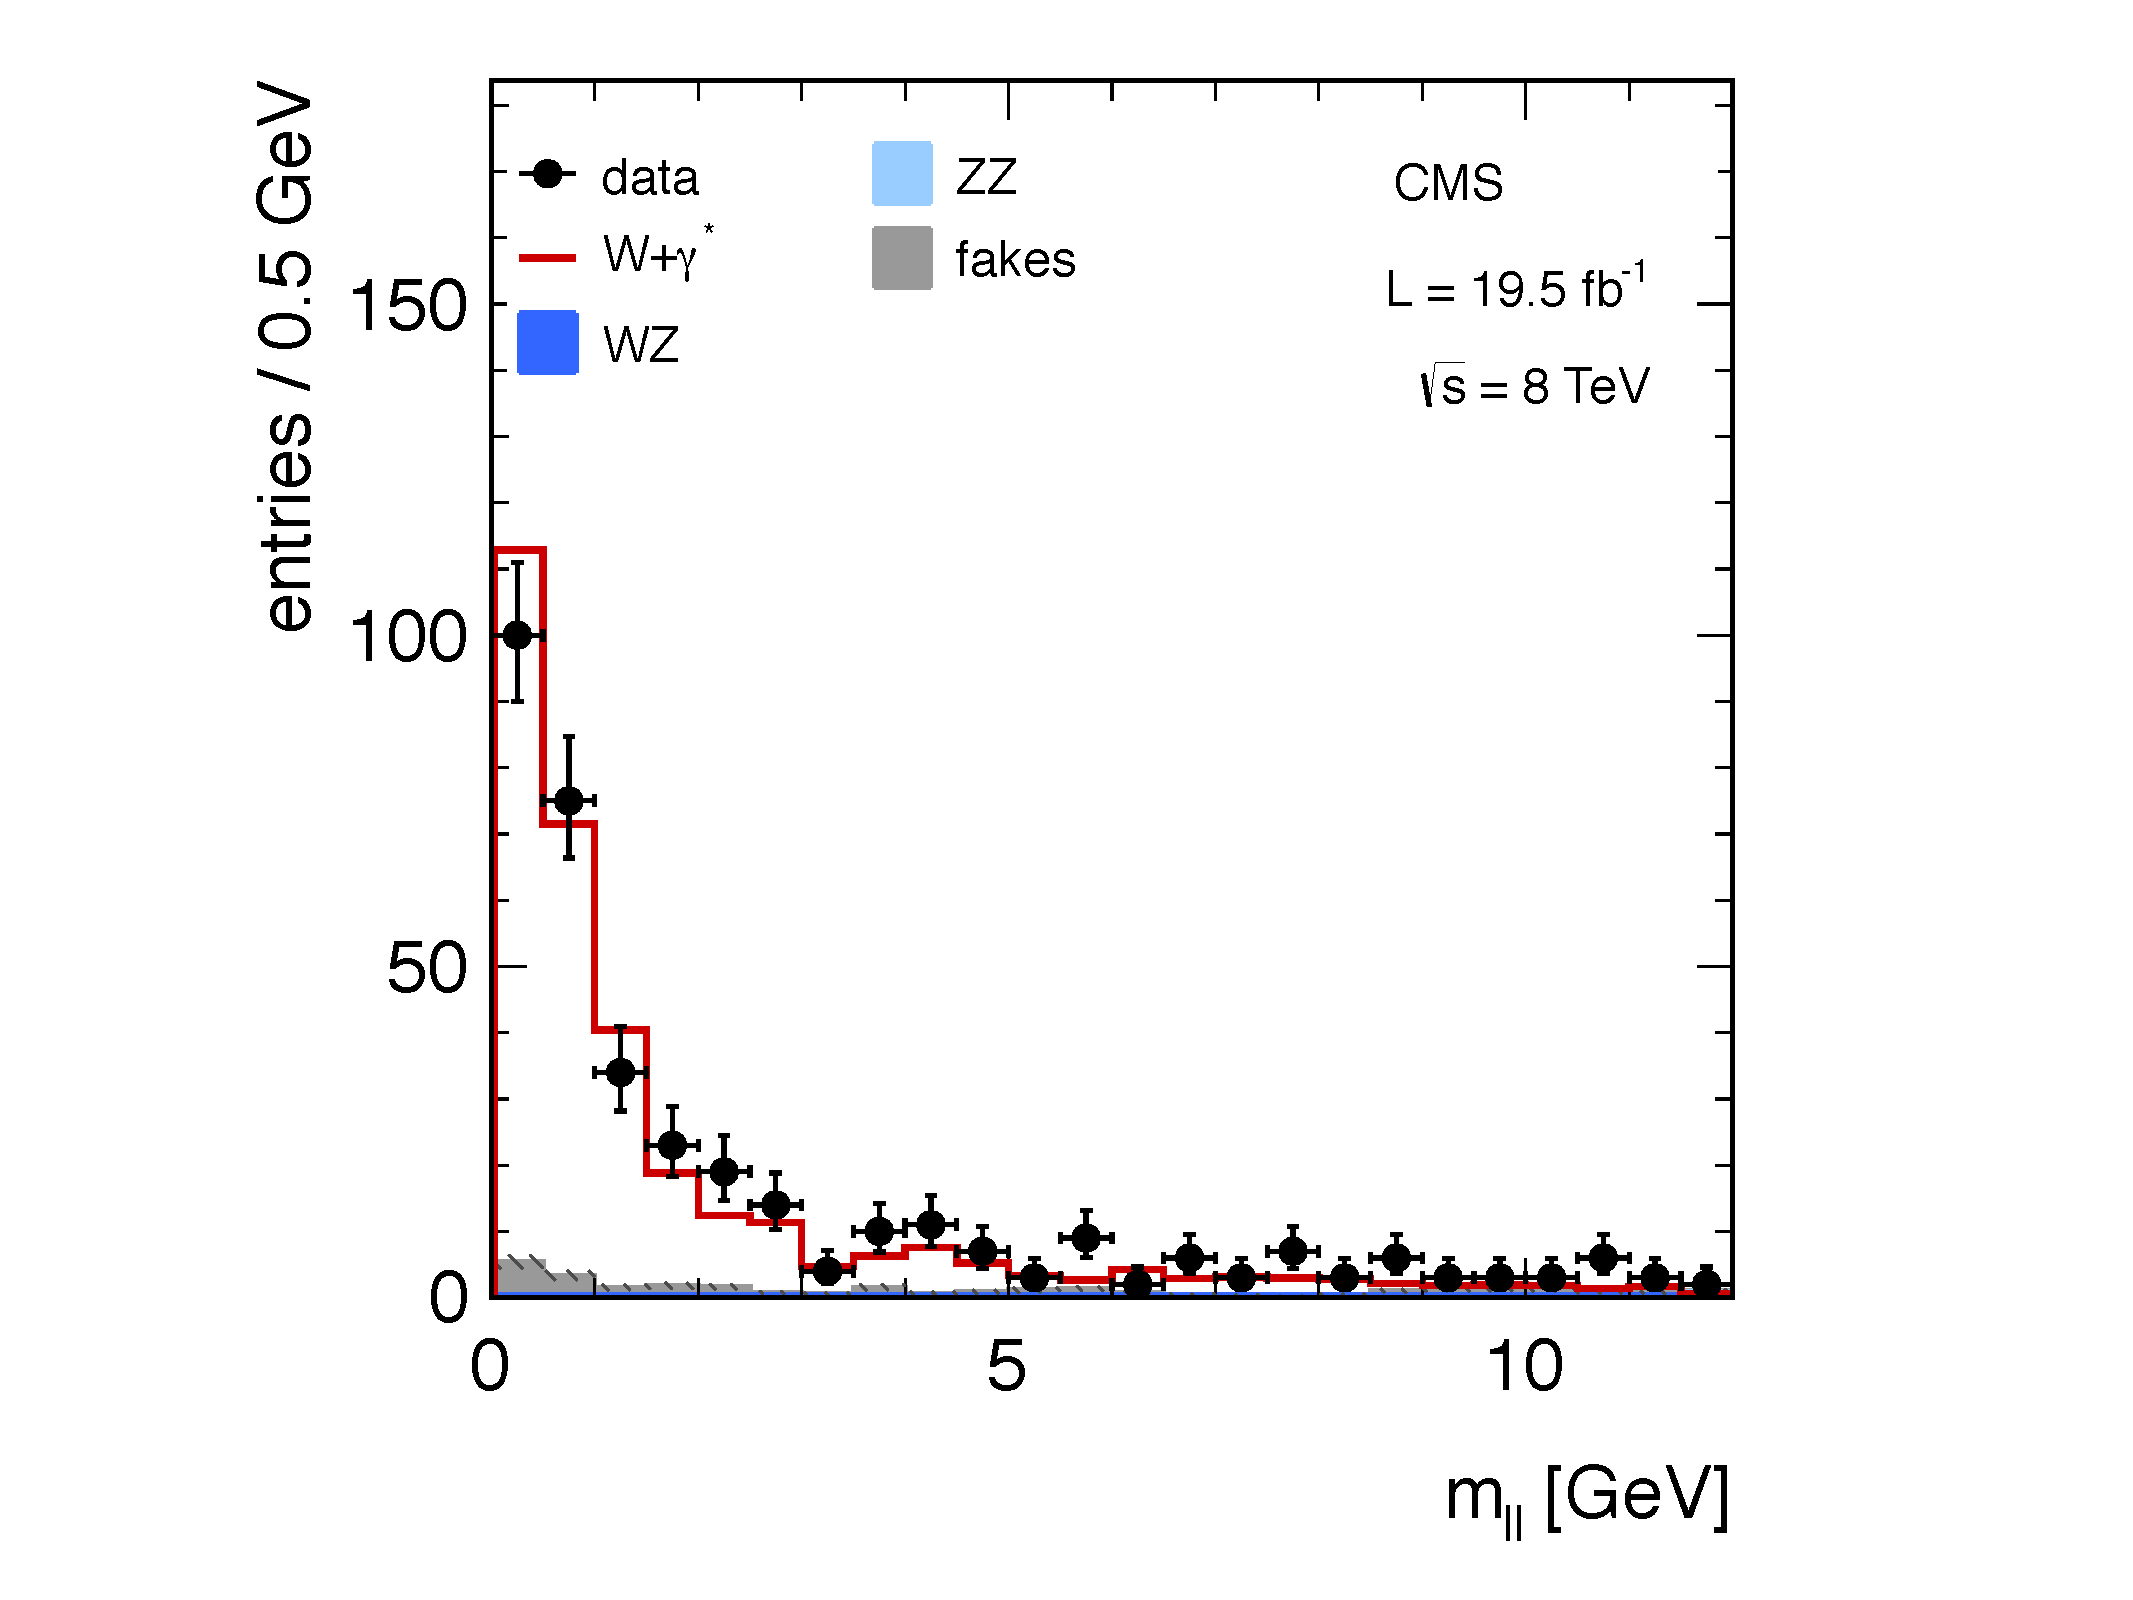
\includegraphics[width=0.8\textwidth]{figures/Wg3l.pdf} 
\end{tabular} 
\caption{\mll\ distribution for opposite-sign muon pairs after \wgammastar\ selection. 
The \wgammastar\ is normalized to match the data.} 
\label{fig:wg3l} 
\end{figure} 

%FIXME : I am here 

%%%%%%%%%%%%%%%%%%%%%%%%%%
\section{ Other backgrounds } 

%%%%%
\subsection{\wgamma}

\wgamma\ can fake signal when the photon converts to a pair of electrons asymmetrically, 
giving a large fraction of its momentum to one electron. The is difficult to measure 
in data, so we rely on simulation after data corrections such as trigger/lepton selection 
efficiencies and PileUp.

For the shape-based analysis, the templates for \wgamma\ suffer from low statistics 
if the full lepton selection is applied for both leptons. So, we take the shape of the 
templates from \wgamma\ events before the photon converts to leptons, and apply 
photon-to-electron conversion probability($P(\gamma \rightarrow e)$) as a function of \Eta. 
The conversion 
factor is measured in simulation and shown in fig.~\ref{fig:photon_electron_ratio}.  
The function is parametrized with \Eta\ because conversion probability has strong 
correlation with the amount of materials that the photon goes through
and it depends on \Eta. 
\begin{figure}[htp] 
\centering 
\begin{tabular}{c} 
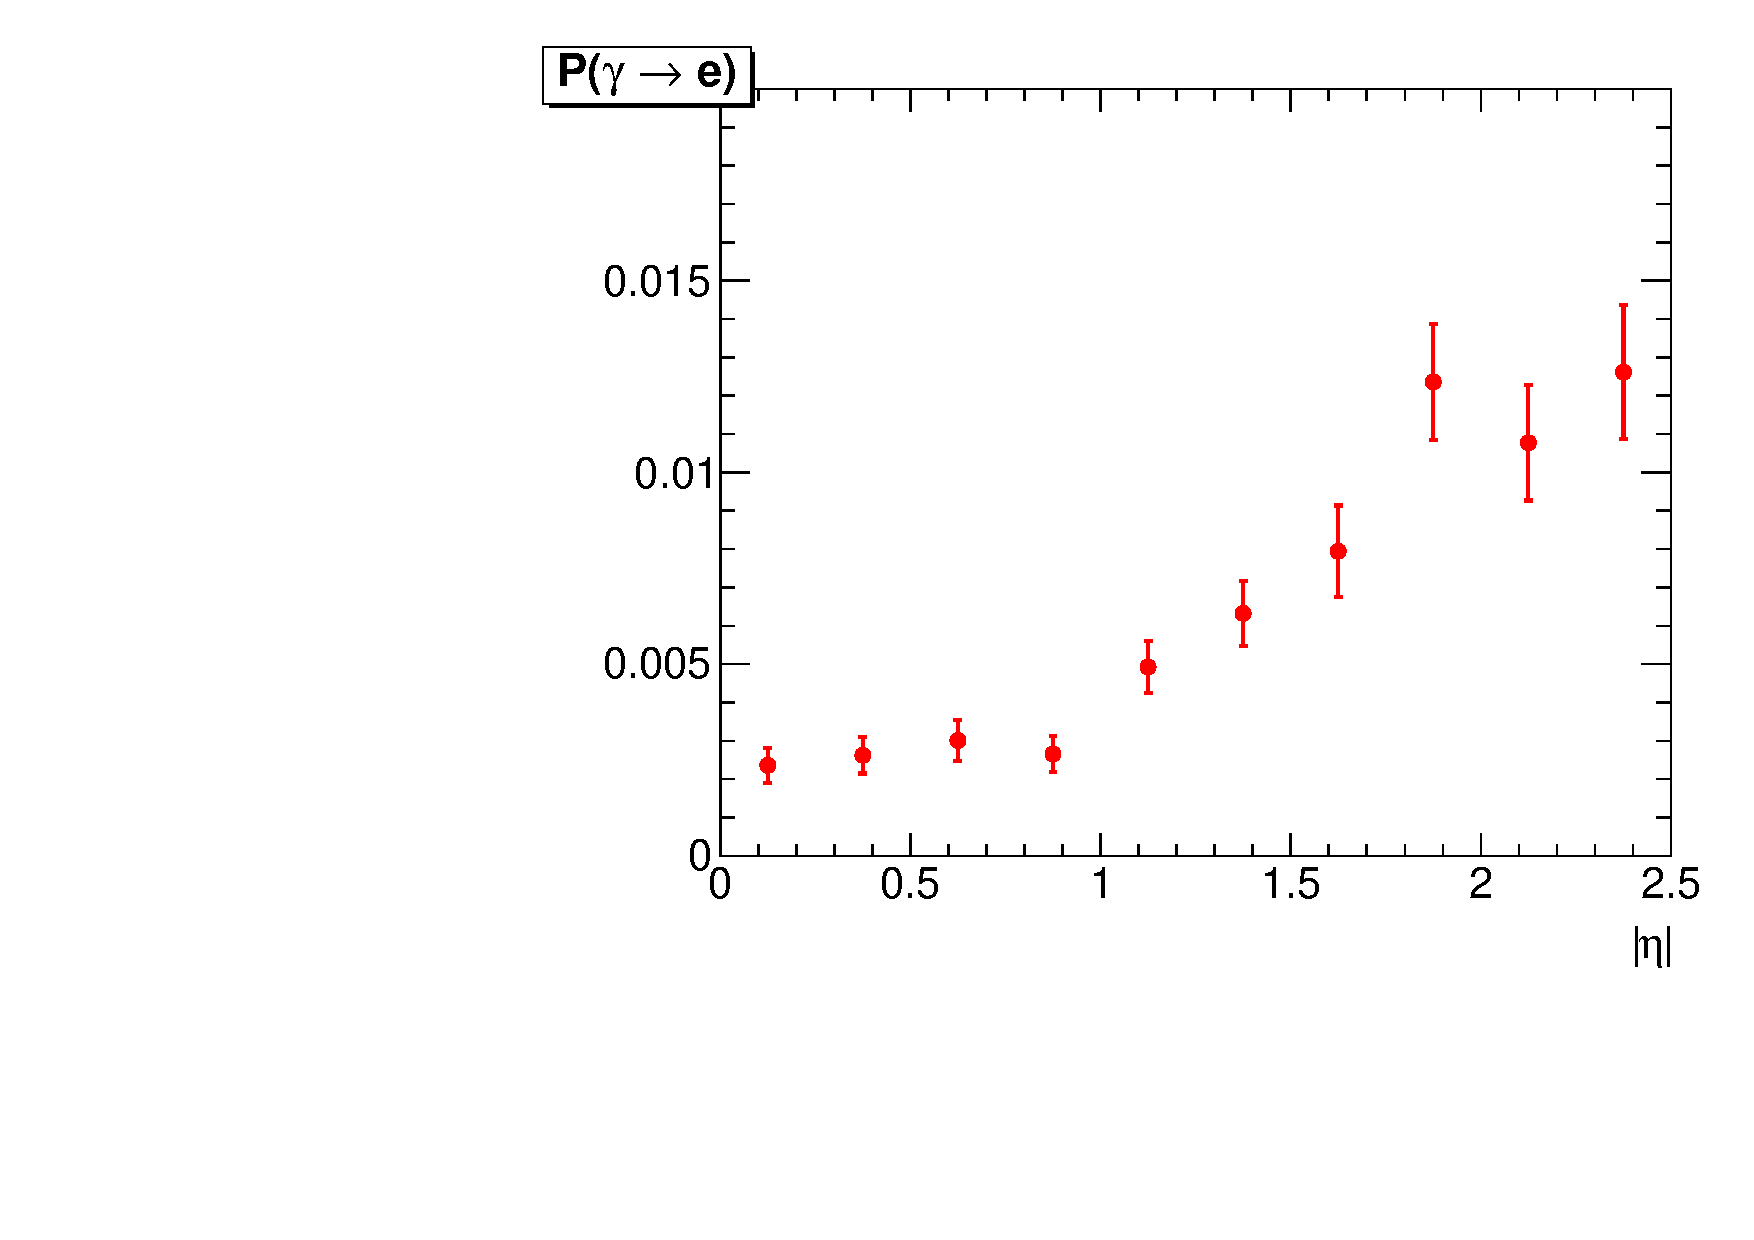
\includegraphics[width=0.7\textwidth]{figures/ratio_photon_electron.pdf} 
\end{tabular} 
\caption{The probability for a photon to convert to a pair of electrons, 
and one of the electrons is selected as a good electron.  } 
\label{fig:photon_electron_ratio} 
\end{figure}  

Fig.~\ref{fig:wgamma_compare} shows the normalized \mll\ and \mt\ distributions 
of \wgamma\ samples, the red is the sample with 2 leptons in the final state 
and black is the sample with 1 lepton + $\gamma$ where the conversion 
factor is applied. The two shapes look consisitent. 
By using the 1 lepton + $\gamma$ sample, we get an order of $\mathcal{O}(10^2)$ 
more statistics in the template.  
\begin{figure}[htp] 
\centering 
\begin{tabular}{c} 
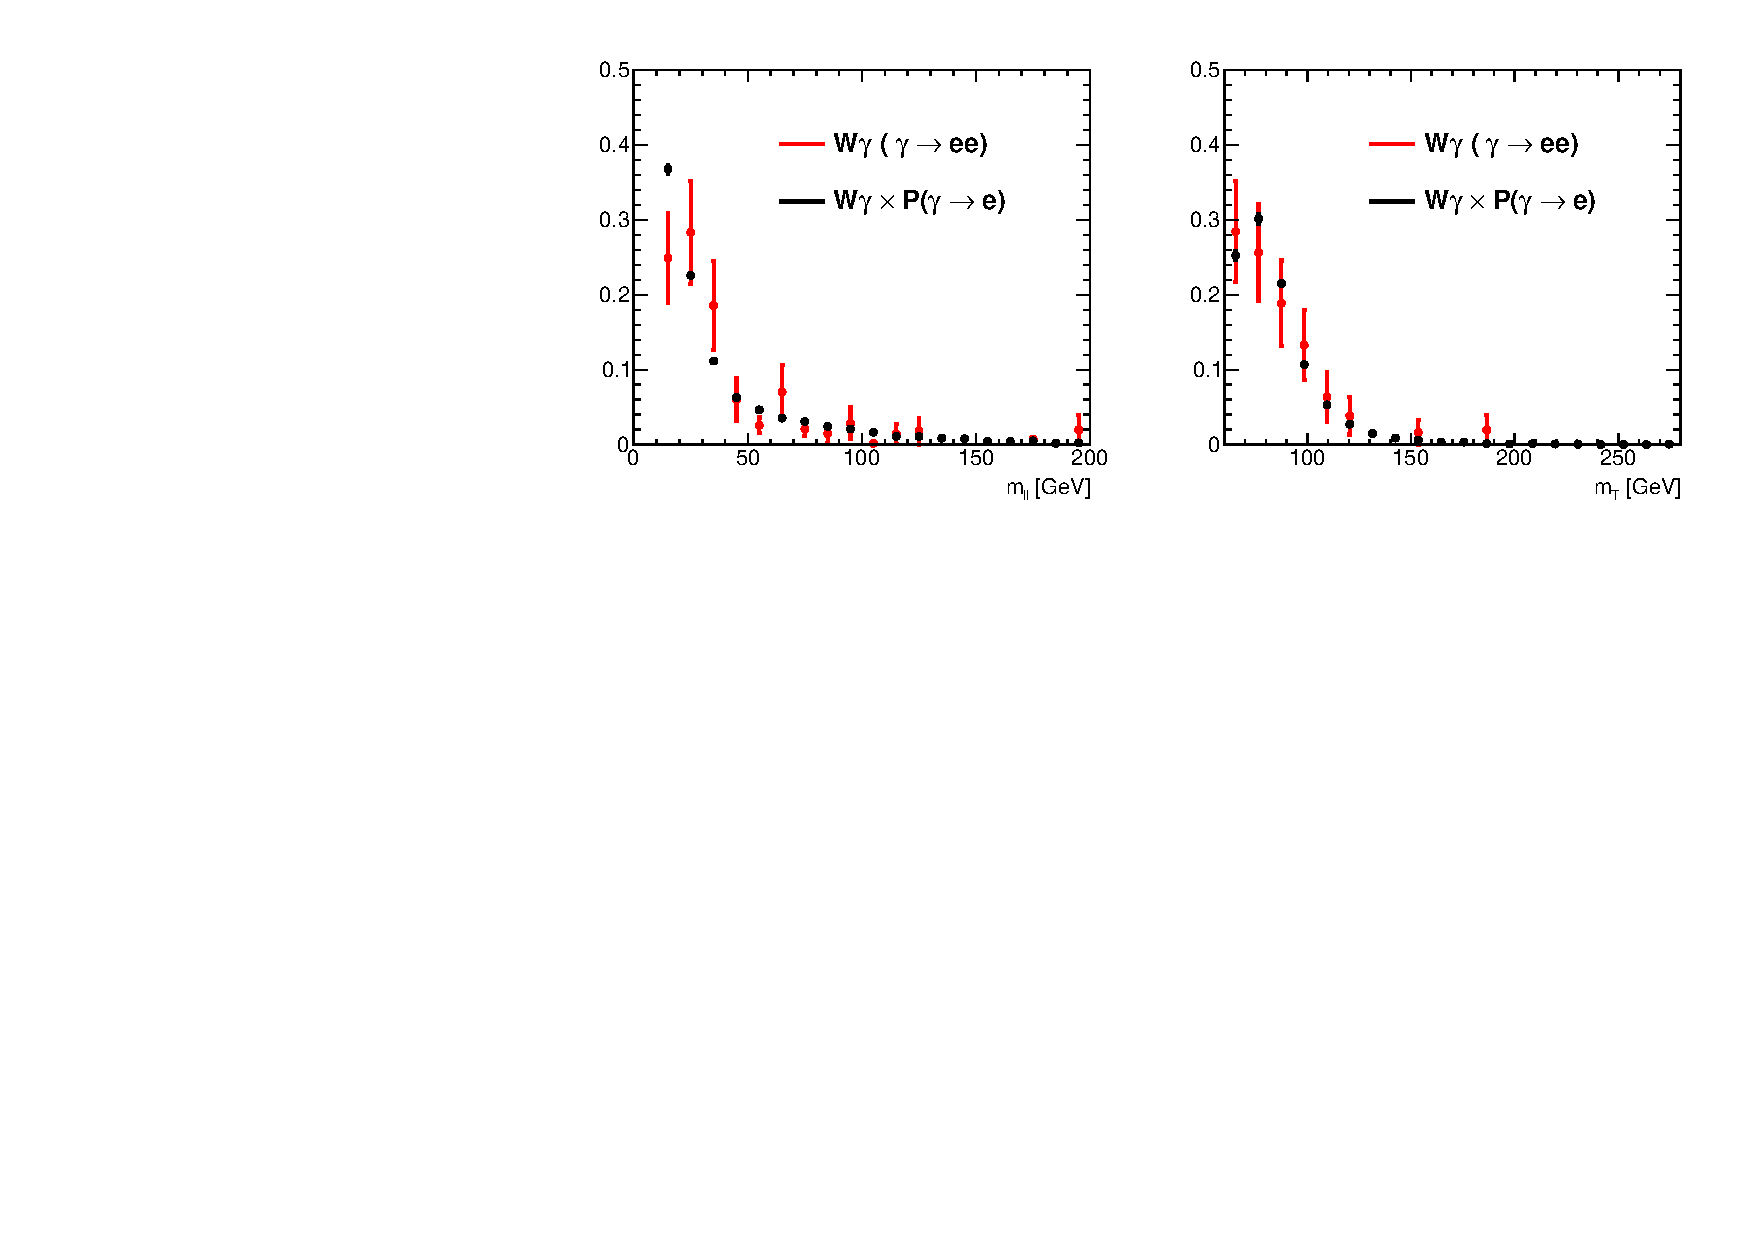
\includegraphics[width=1.0\textwidth]{figures/Wgamma_0j_of.pdf} 
\end{tabular} 
\caption{\mll\ and \mt\ distributions of \wgamma\ samples. 
Red is after photon coverts to electrons and black is before the photon coversion 
with the conversion probability applied. }
\label{fig:wgamma_compare} 
\end{figure}  



%%%%%
\subsection{\ztt}

The \ztt\ background contributes in the \DF\ category in case that 
each of taus decays to a lepton and neutrinos. Typically, the natural source 
of \met\ in \ztt\ gives soft \met\ and met modest \met\ selection can  
reduce this background. But, in the environment of large number of PileUp, 
instrumental contribution to \met\ becomes larger and this leads to large 
\met\ values. The cross section of \ztt\ process is large, so we need to make 
sure that this background is controllable.The simulation does not reproduce 
the instrumental \met properly, and we need a data-driven method to 
accurately estimate \ztt\ background. 

The data-driven method for the estimation of \ztt\ background is done by 
``tau embedding" technique~\cite{}. In this method, we select \dymm\ events in data
from the whole run range, 
and replace each muon with a simulated tau decay, $\tau \rightarrow l\bar{\nu}_l\nu_\tau$. 
Then, the \met\ is re-calculated adding the neutrinos from the tau decays. 
Advantage of this method is that the event environment is taken from the real data, 
and the modeling of PileUp, UE, jets and thus \met\ can be done consistently 
with real data. This sample is normalized to the inclusive \ztt\ MC 
at the level of requiring two leptons with lepton efficiency correction
and the branching fraction.

The 10 \% of systematic uncertainty of the method is assigned based on the MC closure test. 

%%%%%
\subsection{\vv} 

\vv\ backgrounds where the bosons decay leptonically are well-modelled by simulation.
In addition, the contribution of these backgrounds is small. Therefore, to estimate these 
background, we rely on MC after data corrections.  



%%%%%%%%%%%%%%%%%%%%%%%%%%
\section{ The result of background estimation }

The tab.~\ref{tab:wwselection_all} summarizes the result of background estimation. 
It shows the yield of each process in the four final states, 0-jet \SF, 0-jet \DF,  
1-jet \SF and 1-jet \DF.  

\begin{table}[ht!]
\begin{center}
\begin{tabular}{c|c|c|c|c}
\hline
                & \multicolumn{2}{c|}{0-jet}             &          \multicolumn{2}{c}{1-jet}             \\
\hline
                &  \SF                &   \DF             &           \SF     &  \DF               \\
\hline \hline
\qqww           & 1782.4 $\pm$ 11.6        & 4402.1 $\pm$ 18.0 &  533.7 $\pm$  6.0  &  1414.3 $\pm$   9.7 \\
\ggww           &  124.0 $\pm$  2.2        &  223.7 $\pm$  3.0 &        34.1 $\pm$  1.1  &    76.3 $\pm$   1.6 \\
\topbkg         &  273.3 $\pm$  7.8        &  563.7 $\pm$ 11.1 &  677.2 $\pm$ 10.4  &  1644.2 $\pm$  16.8  \\
\wgamma         &   23.5 $\pm$  5.7        &  140.0 $\pm$ 16.9 &        11.9 $\pm$  4.8  &    51.8 $\pm$   9.2 \\
\wgammastar     &   13.7 $\pm$  2.0        &  147.9 $\pm$  6.5 &         2.4 $\pm$  0.8  &    23.9 $\pm$   2.7 \\
%VVV             &   19.8 $\pm$  1.0        &   38.3 $\pm$  1.4 &        16.3 $\pm$  1.5  &    33.4 $\pm$   1.7 \\
%\vv              &   36.8 $\pm$  0.6        &  105.5 $\pm$  1.0 &        23.4 $\pm$  0.5  &   100.7 $\pm$   1.0 \\
\vv              &  56.6 $\pm$  1.2        &  143.8 $\pm$  1.7 &        39.7 $\pm$  1.6  &   134.1 $\pm$   2.0 \\
$\Wjets$        &  107.5 $\pm$  4.6        &  694.8 $\pm$ 10.3 &        47.4 $\pm$  3.6  &   356.2 $\pm$   7.9 \\
$\Zjets$        &  294.6 $\pm$ 60.3        &   82.5 $\pm$  1.4 &  118.4 $\pm$ 30.3  &   248.7 $\pm$   2.8  \\
\hline
Total Bkg.      & 2676.3 $\pm$ 62.5     & 6399.1 $\pm$ 30.1 & 1465.3 $\pm$ 33.3 &   3950.0 $\pm$  23.7   \\
\hline \hline
Data            & 2728                  & 6361                & 1477             & 3944    \\
\hline
\end{tabular}
  \caption{Expected number of signal and background events from the data-driven methods for 
  an integrated luminosity of \intlumiEightTeV after applying the $\WW$ selection requirements. 
  Only statistical uncertainties on the processes are reported.
  $\WW$ yield is from simulation.}
\label{tab:wwselection_all}
\end{center}
\end{table}



and the distributions of relevant kinematic variables. 

